\documentclass[12pt,a4paper]{article}
\usepackage{lmodern}

\usepackage{placeins}
\usepackage{amssymb,amsmath}
\usepackage{ifxetex,ifluatex}
\usepackage{fixltx2e} % provides \textsubscript
\ifnum 0\ifxetex 1\fi\ifluatex 1\fi=0 % if pdftex
  \usepackage[T1]{fontenc}
  \usepackage[utf8]{inputenc}
\else % if luatex or xelatex
  \ifxetex
    \usepackage{mathspec}
    \usepackage{xltxtra,xunicode}
  \else
    \usepackage{fontspec}
  \fi
  \defaultfontfeatures{Mapping=tex-text,Scale=MatchLowercase}
  \newcommand{\euro}{€}
\fi
% use upquote if available, for straight quotes in verbatim environments
\IfFileExists{upquote.sty}{\usepackage{upquote}}{}
% use microtype if available
\IfFileExists{microtype.sty}{%
\usepackage{microtype}
\UseMicrotypeSet[protrusion]{basicmath} % disable protrusion for tt fonts
}{}
\usepackage[lmargin = 5cm,rmargin = 2.5cm,tmargin = 2.5cm,bmargin = 2.5cm]{geometry}

% Figure Placement:
\usepackage{float}
\let\origfigure\figure
\let\endorigfigure\endfigure
\renewenvironment{figure}[1][2] {
    \expandafter\origfigure\expandafter[H]
} {
    \endorigfigure
}

%%%% Jens %%%%
\DeclareMathOperator*{\argmax}{arg\,max}
\DeclareMathOperator*{\argmin}{arg\,min}

\usepackage{numprint}
\npthousandsep{\,}

%% citation setup
\usepackage{csquotes}

\usepackage[backend=biber, maxbibnames = 99, style = apa]{biblatex}
\setlength\bibitemsep{1.5\itemsep}
\addbibresource{R_packages.bib}
\bibliography{references.bib}
\usepackage{graphicx}
\makeatletter
\def\maxwidth{\ifdim\Gin@nat@width>\linewidth\linewidth\else\Gin@nat@width\fi}
\def\maxheight{\ifdim\Gin@nat@height>\textheight\textheight\else\Gin@nat@height\fi}
\makeatother
% Scale images if necessary, so that they will not overflow the page
% margins by default, and it is still possible to overwrite the defaults
% using explicit options in \includegraphics[width, height, ...]{}
\setkeys{Gin}{width=\maxwidth,height=\maxheight,keepaspectratio}
\ifxetex
  \usepackage[setpagesize=false, % page size defined by xetex
              unicode=false, % unicode breaks when used with xetex
              xetex]{hyperref}
\else
  \usepackage[unicode=true, linktocpage = TRUE]{hyperref}
\fi
\hypersetup{breaklinks=true,
            bookmarks=true,
            pdfauthor={Jens Klenke},
            pdftitle={Analysing FIFA Data with the Bayesian LASSO},
            colorlinks=true,
            citecolor=black,
            urlcolor=black,
            linkcolor=black,
            pdfborder={0 0 0}}
\urlstyle{same}  % don't use monospace font for urls
\setlength{\parindent}{0pt}
\setlength{\parskip}{6pt plus 2pt minus 1pt}
\setlength{\emergencystretch}{3em}  % prevent overfull lines
\setcounter{secnumdepth}{5}

%%% Use protect on footnotes to avoid problems with footnotes in titles
\let\rmarkdownfootnote\footnote%
\def\footnote{\protect\rmarkdownfootnote}

%%% Change title format to be more compact
\usepackage{titling}

% Create subtitle command for use in maketitle
\newcommand{\subtitle}[1]{
  \posttitle{
    \begin{center}\large#1\end{center}
    }
}

\setlength{\droptitle}{-2em}
  \title{Analysing FIFA Data with the Bayesian LASSO}
  \pretitle{\vspace{\droptitle}\centering\huge}
  \posttitle{\par}
\subtitle{Seminar in Econometrics}
  \author{Jens Klenke}
  \preauthor{\centering\large\emph}
  \postauthor{\par}
  \predate{\centering\large\emph}
  \postdate{\par}
  \date{today}

\usepackage{booktabs}
\usepackage{longtable}
\usepackage{array}
\usepackage{multirow}
\usepackage{wrapfig}
\usepackage{float}
\usepackage{colortbl}
\usepackage{pdflscape}
\usepackage{tabu}
\usepackage{threeparttable}
\usepackage{threeparttablex}
\usepackage[normalem]{ulem}
\usepackage{makecell}
\usepackage{xcolor}

%% linespread settings

\usepackage{setspace}

\onehalfspacing

% Language Setup

\usepackage{ifthen}
\usepackage{iflang}
\usepackage[super]{nth}
\usepackage[ngerman, english]{babel}

%Acronyms
\usepackage[printonlyused, withpage, nohyperlinks]{acronym}
\usepackage{changepage}

% Multicols for the Title page
\usepackage{multicol}

\begin{document}

\selectlanguage{english}

%%%%%%%%%%%%%% Jens %%%%%
\numberwithin{equation}{section}


%\maketitle

\begin{titlepage}
  \noindent\begin{minipage}{0.6\textwidth}
	  \IfLanguageName{english}{University of Duisburg-Essen}{Universität Duisburg-Essen}\\
	  \IfLanguageName{english}{Faculty of Business Administration and Economics}{Fakultät für Wirtschaftswissensschaften}\\
	  \IfLanguageName{english}{Chair of Econometrics}{Lehrstuhl für Ökonometrie}\\
  \end{minipage}
	\begin{minipage}{0.4\textwidth}
	  \begin{flushright}
  	  \vspace{-0.5cm}
      \IfLanguageName{english}{\includegraphics*[width=5cm]{Includes/duelogo_en.png}}{\includegraphics*[width=5cm]{Includes/duelogo_de.png}}
	  \end{flushright}
	\end{minipage}
  \\
  \vspace{0.25cm}
  \begin{center}
  \huge{Analysing FIFA Data with the Bayesian LASSO}\\
  \vspace{.25cm}
  \Large{Seminar in Econometrics}\\
  \vspace{0.5cm}
  \large{Term Paper}\\
  \vspace{0.5cm}
  \large{  \IfLanguageName{english}{Submitted to the Faculty of \\  Business Administration and Economics  \\at the \\University of Duisburg-Essen}{Vorgelegt der \\Fakultät für Wirtschaftswissenschaften der \\ Universität Duisburg-Essen}\\}
  \vspace{0.75cm}
  \large{\IfLanguageName{english}{from:}{von:}}\\
  \vspace{0.5cm}
  Jens Klenke\\
  \end{center}
  %\vspace{2cm}
  \vfill
  \hrulefill

  \noindent\begin{minipage}[t]{0.3\textwidth}
  \IfLanguageName{english}{Reviewer:}{Erstgutachter:}
  \end{minipage}
  \begin{minipage}[t]{0.7\textwidth}
  \hspace{1cm}Christoph Hanck
  \end{minipage}

  \noindent\begin{minipage}[t]{0.3\textwidth}
  \IfLanguageName{english}{Deadline:}{Abgabefrist:}
  \end{minipage}
  \begin{minipage}[t]{0.7\textwidth}
  \hspace{1cm}Jan.~17th 2020
  \end{minipage}

  \hrulefill

  \begin{multicols}{2}

  Name:

  Matriculation Number:

  E-Mail:

  Study Path:

  Semester:

  Graduation (est.):
 
  \columnbreak

  Jens Klenke

  3071594
  
  jens.klenke@stud.uni-due.de

  M.Sc. Economics

  \nth{5}

  Winter Term 2020

	\end{multicols}

\end{titlepage}

\newgeometry{top=2cm, left = 5cm, right = 2.5cm, bottom = 2.5cm}


\pagenumbering{Roman}
{
\hypersetup{linkcolor=black}

\setcounter{tocdepth}{3}
\tableofcontents
}

\newpage
\listoffigures
\addcontentsline{toc}{section}{List of Figures}

%\newpage
\listoftables
\addcontentsline{toc}{section}{List of Tables}

\section*{List of Abbreviations}
\addcontentsline{toc}{section}{List of Abbreviations}

\begin{adjustwidth}{1.5em}{0pt}

\begin{acronym}[dummyyyy]
 \acro{bagging}{Bootstrap Aggregation}
 \acro{LASSO}{Least Absolute Shrinkage and Selection Operator}
 \acro{OLS}{ordinary least squares}
 \acro{pcr}{Principal Components Regression}
 \acro{pls}{Partial Least Squares}
 \acro{RMSE}{Root Mean Squared Error}
 \acro{MCMC}{Markov chain Monte Carlo} 
 \acro{i.i.d.}{independent and identically distributed}
 \acroplural{LRG}[LRG]{längefristige Refinanzierungsgeschäfte}

%Falls eine Abkürzung in der Mehrzahl nicht einfach auf "s" endet muss das speziell eingestellt werden.
% \acro{slmtA}{super lange mega tolle Abkürzung} %Einzahl
 %\acroplural{slmtA}[slmtAs]{super lange mega tolle Abkürzungen} %Mehrzahl
 \acro{dummyyyy}{dummyyy}
\end{acronym}

\end{adjustwidth}

\restoregeometry

\newpage
\pagenumbering{arabic} %Roman arabic

\hypertarget{introduction}{%
\section{Introduction}\label{introduction}}

In recent years, the \ac{LASSO} method by
\textcite{tibshirani_regression_1996} has emerged as an alternative to
ordinary least squares estimation. The success of the method is mainly
due to its ability to perform both variable selection and estimation. As
Tibshirani already pointed out in his original paper the standard
\ac{LASSO} model can be interpreted as a linear regression with a
Laplace prior. \textcite{park_bayesian_2008} were the first to implement
the Bayesian \ac{LASSO} \textgreater\textgreater using a conditional
Laplace prior specification\textless\textless.

Our goal is to compare the results of the Bayesian \ac{LASSO} with the
normal \ac{LASSO} method and an ordinary least square estimation. The
focus is particularly on the number of non-significant parameters in the
linear model or, in case of the \acp{LASSO} the parameters equal to
zero. To compare the different methods we will use the FIFA data sets
from 2019 and 2020.

Bayesian statistics has grown very strongly in recent years. This is due
to the improvement of computers which have made the calculation possible
in the first place. Now they make it possible to calculate these methods
in increasing numbers and in even shorter time. In view of these
changes, it seems logical that the Bayesian LASSO should be used more
and more often, since this method can select variables and also estimate
variables by means of distributions. This leads to the fact that the
advantages of LASSO and Bayesian statistics come together. Nevertheless,
the Bayesian methods still take much longer to calculate than the
frequentist methods. Therefore, in this paper we want to analyze whether
the Bayesian LASSO has an advantage over the frequentist LASSO.

In the first chapter we will present the general approach of Bayesian
statistics. Afterwards, we will describe the data basis and preparation.
The next step is to introduce the methods used and to present the
results. Before we will draw a conclusion, the models will be analyzed
with respect to their residuals.

\newpage

\hypertarget{theory-of-bayesian-inference}{%
\section{Theory of Bayesian
inference}\label{theory-of-bayesian-inference}}

The Bayesian (inference) statistics based on the Bayes' theorem for
events.

\begin{align}
\label{eq:bayes_theorem}
  P(A | B) = \dfrac{P (B | A) P(A)}{P(B)}
\end{align}

For Bayesian statistics the event theorem \eqref{eq:bayes_theorem} gets
rewritten to apply it to densities.

Where \(\pi (\theta)\) is the prior distribution - which could be gained
from prior research or knowledge, \(f(y | \theta )\) is the likelihood
function, and \(\pi (\theta| y)\) is the posterior distribution, which
then yields in the following equation:

\begin{align}
\label{eq:bayes_dens}
  \pi (\theta | y) = \dfrac{f(y | \theta) \pi(\theta)}{f(y)}
\end{align}

From equation \eqref{eq:bayes_dens} the advantages and disadvantages of
Bayesian statistics compared to frequentist statistics can directly be
retrieved. One major advantage is that the Bayesian approach can account
for prior knowledge and points out a philosophical difference to the
frequentist approach - that the obtained data stands not alone.

Another key difference and advantage is that in the Bayesian statistic
the computations are made with distributions and this leads to a better
information level than just the computation of the first and second
moment.

The computation with distributions is also the greatest disadvantage or
- more neutral - the biggest problem of the Bayesian approach because in
high dimensional problems the computation takes a lot of time and in
some cases it is even impossible. A solution to that is that with newer
and better computers it is possible to simulate the integrals with a
\ac{MCMC} method. \autocite[p.~35 ff.]{ghosh_introduction_2006}

\newpage

\hypertarget{data-description}{%
\section{Data description}\label{data-description}}

We collected the data from the online database platform \emph{kaggel.}
The dataset includes 6 years of data for all players who were included
in the soccer simulation game \emph{FIFA} from \emph{EA Sports}. We
decided to keep the data for 2019 and 2020, only. The Data for 2019
contains 17538 datapoints which will be used for the estimation of the
different models whereas the 2020 data with 18028 will be used to
compare the quality of the models with an out of sample \ac{RMSE}. Both
datasets consist of 104 variables which will not all be included in the
estimations. Some Variables are just an ID or different length of names
and URLs. \autocite{leone_fifa_2020}

A fundamental problem of the dataset consists as goalkeepers are
systematically rated differently than field players. Therefore, in the
subcategories of the variable \emph{overall} all field player categories
were assigned NAs for goalkeepers. Conversely, all field players have
NAs in all goalkeeper categories. Because the algorithm of \ac{LASSO} in
R cannot handle NAs they have been set to zero for all models.

It is not very realistic that a fielder has no values in the goalkeeper
categories and vice versa. However, it can be argued, at least for
outfield players, that goalkeeper attributes play no role in determining
market values. This argumentation does not seem to hold for goalkeepers,
at least passing can be assumed to be an influential variable for the
market value, because is an essential asset for the passing game if the
goalkeeper has possession of the ball. Nevertheless, due to the lack of
alternatives, all NAs have been replaced by Zero.

\begin{table}[!h]

\caption{\label{tab:data}\label{tab:sum} Summary of some important variables for the 2019 FIFA edition}
\centering
\begin{tabular}[t]{lllrlrr}
\toprule
 & year &  & N &   & mean & sd\\
\midrule
\rowcolor{gray!6}  value\_eur & 2019 &  & 17 538 &  & 2 473 043.68 & 5 674 963.22\\
 & 2020 &  & 18 028 &  & 2 518 484.58 & 5 616 359.21\\
\rowcolor{gray!6}  wage\_eur & 2019 &  & 17 538 &  & 10 085.87 & 22 448.70\\
 & 2020 &  & 18 028 &  & 9 584.81 & 21 470.29\\
\rowcolor{gray!6}  overall & 2019 &  & 17 538 &  & 66.23 & 7.01\\
 & 2020 &  & 18 028 &  & 66.21 & 6.95\\
\rowcolor{gray!6}  age & 2019 &  & 17 538 &  & 25.17 & 4.64\\
 & 2020 &  & 18 028 &  & 25.23 & 4.63\\
\rowcolor{gray!6}  potential & 2019 &  & 17 538 &  & 71.40 & 6.15\\
 & 2020 &  & 18 028 &  & 71.56 & 6.14\\
\bottomrule
\end{tabular}
\end{table}

As one can see in Table \ref{tab:sum} the differences between the
editions for the most important variables are considerably small.

For example, from 2019 to 2020 the mean player \emph{value} (response
variable) increased by 4.54e+04 which is about 1.8 per cent or 0.01
standard deviations. Similar results are observable for the probably
most important righthand variables \emph{wage} and \emph{overall} with a
difference in the means of -0.02 and -0.003 standard deviations between
2019 and 2020.

\begin{figure}
\centering
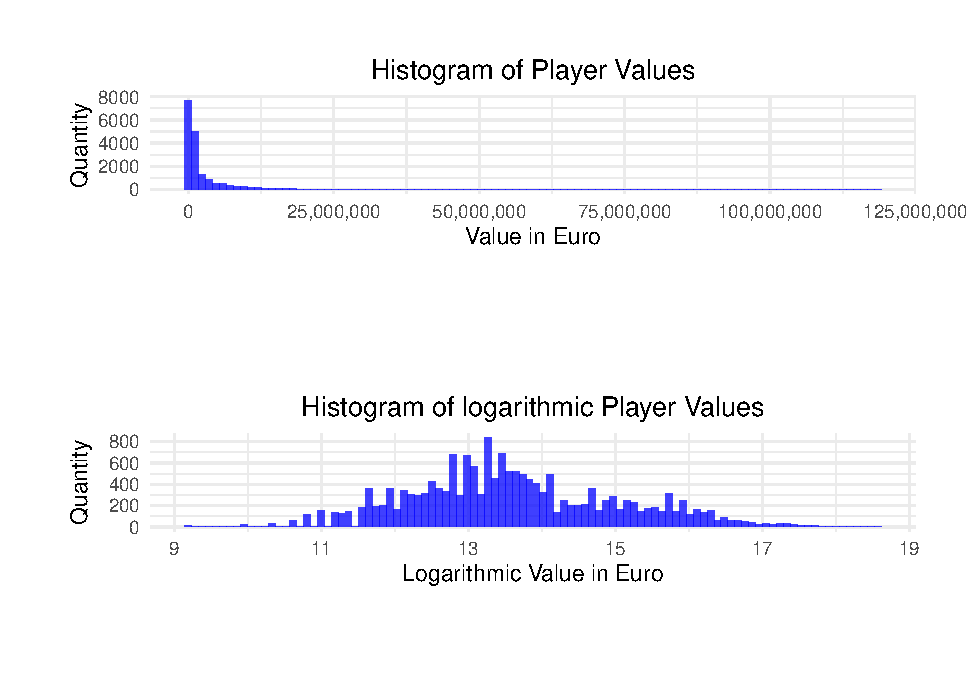
\includegraphics{term_paper_bayes_files/figure-latex/fig1-1.pdf}
\caption{\label{fig:hist_1} Histograms of player values and log player
values}
\end{figure}

As can be seen for the variable \emph{value} in Figure \ref{fig:hist_1},
this relatively strong right-skew is distributed, a similar pattern can
be observed for the variable wage. Since we also have estimate a linear
model, and this often leads to non-normally distributed residuals, these
were logarithmized.

\newpage

\hypertarget{used-models}{%
\section{Used Models}\label{used-models}}

To compare the Bayesian \ac{LASSO} we will also analyze the data with a
linear multivariate model, and the frequentist \ac{LASSO}. We will start
with the linear model and then gradually modify the model equations
respectively the condition for estimating the parameters. So that the
coherences between the individual methods become clear.

All three methods have the common assumption that the relationship is
linear, at least in the parameters. Inatially, the assumption seems
stricter than it is, because the data can be manipulated in such a way
that the relationship is linear after all. In our data this was done by
logarithmization.

\hypertarget{linear-model}{%
\subsection{Linear Model}\label{linear-model}}

The frequentist multivariate regression model has the following model
equation.

\begin{align}
\label{eq:lm}
\pmb{Y = \beta_0 + X \beta} + \pmb{\epsilon}
\end{align}

Where \(\pmb{y}\) is the \(n \times 1\) response vector, \(\pmb{X}\) is
the \(n \times p\) matrix of regressors and, \(\pmb{\epsilon}\) is the
\(n \times 1\) vector of \ac{i.i.d.} errors with mean 0 and unknown but
constant variance \(\sigma^2\).

The coefficient will be estimated by the ordinary least square method,
which means that \(\pmb{\beta}\) should be chosen so that the
\emph{Euclidean norm} \(\left( || \mathbf{y - X\beta} ||_2 \right)\) is
minimal. This yields in the condition for the estimation of
coefficients:

\begin{align}
\label{eq:lm_con}
 \hat{\pmb{\beta}} = \argmin_{ \pmb{\beta}} (\pmb{y - \beta_0 - X  \beta})^T (\pmb{y - \beta_0 - X  \beta})
\end{align}

\hypertarget{section}{%
\subsection{\texorpdfstring{\acf{LASSO}}{}}\label{section}}

In the \ac{LASSO} method the model equation is the same as the equation
for the multivariate but the condition for the optimization of the
estimators in equation \eqref{eq:lm_con} has an additional punishment
term. Which leads to the following optimization.

\begin{align}
\label{eq:la_con}
\hat{\pmb{\beta}} = \argmin_{\pmb{\beta}}  \left( \pmb{y - X \beta} \right)^T \left( \pmb{y - X \beta} \right) + \lambda \sum_{i = 1}^{p} |\beta_j|
\end{align}

for some \(\lambda \geq 0\). This method is also often referred to as
\(L_1\) -penalized least squares estimation.

Already in his original paper \textcite{tibshirani_regression_1996} has
pointed out the possibility that his methods can also be interpreted in
a Bayesian way. The LASSO estimates can be considered as posterior mode
estimates with a double-exponential Laplace prior.

\hypertarget{bayesian-lasso}{%
\subsection{Bayesian Lasso}\label{bayesian-lasso}}

\textcite{park_bayesian_2008} considered a fully Bayesian approach using
a conditional Laplace prior of the form

\begin{align} 
\label{eq:la_bay_prior}
 \pi \left( \pmb{\beta} | \sigma^2 \right)   = \prod_{j = 1}^{p} \dfrac{\lambda}{2 \sqrt{\sigma^e}} e^{\dfrac{- \lambda |\beta_j |}{\sqrt{\sigma^2}}} 
\end{align}

The analysis of the FIFA data set is a multidimensional problem and
therefore in Bayesian statistics this is an analysis that only works
with a hierarchical model. The solution cannot be calculated directly
but has to be solved with the Gibbs sampler.

\hypertarget{gibbs-sampler}{%
\subsubsection{Gibbs Sampler}\label{gibbs-sampler}}

The Gibbs Sampler is a special case of an \ac{MCMC} algorithm, which is
useful to approximate the combined distribution of two or more
regressors in a multidimensional problem.

The algorithm tries to find the approximate joint distribution and
therefore the algorithm runs through the sub-vectors of \(\beta\) and
draws each subset conditional on all other values.
\autocite{gelman_bayesian_2004}

\newpage

In the \textbf{monomvn} package in \textbf{R}
\autocite{gramacy_monomvn_2019} the Gibbs sampler for the Bayesian
\ac{LASSO} samples from the following representation of the Laplace
distribution. \textcite{andrews_scale_1974}

\begin{align} 
\label{eq:gibbs}
  \dfrac{a}{2}e^{-a |z|} = \int_{0}^{\infty} \dfrac{1}{2 \sqrt{\sigma^2}} e^{ -z^2 / (2s)} \; \dfrac{a^2}{2} e^{ -a^2 s /2} ds, \qquad a > 0 
\end{align}

\hypertarget{the-full-model-specification}{%
\subsubsection{The full Model
specification}\label{the-full-model-specification}}

The full model has the following hierarchical representation

\begin{align*}
  \pmb{y|\mu}, \pmb{X}, \pmb{\beta}, \sigma^2 & \sim N_n (\mu \pmb{1}_n + \pmb{X \beta}, \sigma^2  \pmb{I}_n)   \nonumber\\
  \pmb{\beta} | \sigma^2, \tau^2_1 , \ldots , \tau^2_p & \sim N_p (\pmb{A}^{-1} \pmb{X}^T \tilde{\pmb{y}}  , \sigma^2 \pmb{A}^{-1}) \qquad \text{with} \; \pmb{A} = \pmb{X}^T \pmb{X} + \pmb{D}^{-1}_{\tau} \nonumber \\
  \pmb{D}_{\tau} & = diag(\tau^2_1 , \ldots , \tau^2_p) \nonumber \\ 
  \sigma^2, \tau^2_1 , \ldots , \tau^2_p & \sim \pi \left( \sigma^2 \right) d \sigma^2 \prod_{j = 1}^{p} \dfrac{\lambda^2}{2}e^{- \lambda^2 \tau^2_j /2} d \tau^2_j \nonumber \\
  \sigma^2, \tau^2_1 , \ldots , \tau^2_p & > 0 \nonumber \\
\end{align*}

If \(\tau^2_1 , \ldots , \tau^2_p\) gets integrated out of the
conditional prior on \(\pmb{\beta}\) , we get the form of
\eqref{eq:la_bay_prior}. For \(\sigma^2\) the inverse-gamma function of
the form \(\pi \left( \sigma^2 \right) = \dfrac{1}{\sigma^2}\) was
implemented in the \textbf{monomvn} package.

\newpage

\hypertarget{estimation-and-results-of-the-models}{%
\section{Estimation and Results of the
Models}\label{estimation-and-results-of-the-models}}

To compare the performances of the models all three models got,
obviously, estimated with the same regressors. We included as righthand
variables: \emph{log\_wage} , \emph{age}, \emph{height\_cm},
\emph{weight\_kg}, \emph{overall}, \emph{potential}, \emph{shooting},
\emph{contract\_valid\_until}, \emph{pace}, \emph{passing},
\emph{dribbling}, and \emph{defending}, so we have 12 explanatory
variables to predict the response variable \emph{log\_value}.

The reason we chose relatively few variables is that, on the one hand,
we have enough variables, so it is very likely that some variables will
not become significant, but on the other hand, we also have a better
overview of the variables.

Of course, this can lead to biases in the parameters, but the aim of the
work is not to provide a causal interpretation of the explanatory
variables, but rather to compare the methods.

\hypertarget{linear-model-1}{%
\subsection{Linear Model}\label{linear-model-1}}

\FloatBarrier
\begin{table}[!h]

\caption{\label{tab:structure and lm}\label{tab:sum_lm} Summary of the linear model}
\centering
\begin{tabular}[t]{lrrrr}
\toprule
  & Estimate & Std. Error & t value & Pr(>|t|)\\
\midrule
\rowcolor{gray!6}  (Intercept) & -8.5970 & 2.9222 & -2.9420 & 0.0033\\
log\_wage & 0.0679 & 0.0025 & 26.8466 & 0.0000\\
\rowcolor{gray!6}  age & -0.1004 & 0.0008 & -119.6665 & 0.0000\\
height\_cm & 0.0012 & 0.0004 & 2.7140 & 0.0067\\
\rowcolor{gray!6}  weight\_kg & 0.0001 & 0.0004 & 0.3175 & 0.7508\\
overall & 0.2098 & 0.0008 & 266.5231 & 0.0000\\
\rowcolor{gray!6}  potential & -0.0059 & 0.0007 & -8.1962 & 0.0000\\
shooting & 0.0049 & 0.0003 & 17.7691 & 0.0000\\
\rowcolor{gray!6}  contract\_valid\_until & 0.0051 & 0.0014 & 3.5164 & 0.0004\\
pace & 0.0008 & 0.0002 & 3.6118 & 0.0003\\
\rowcolor{gray!6}  passing & 0.0019 & 0.0004 & 4.5131 & 0.0000\\
dribbling & -0.0016 & 0.0005 & -3.4678 & 0.0005\\
\rowcolor{gray!6}  defending & -0.0017 & 0.0002 & -10.6851 & 0.0000\\
\bottomrule
\end{tabular}
\end{table}
\FloatBarrier

In Table \ref{tab:sum_lm} one can see that only 1 parameter
\emph{weight\_kg} is not significant to a 5 per cent level. The variable
\emph{overall} has, naturally, the biggest (positive) impact on the
\emph{log\_value (value)}, whereas \emph{age} has the biggest negative
effect.

\begin{align} 
\label{eq:t_test}
  t = \dfrac{\beta_i - 0}{se \left( \beta_i \right)} = \dfrac{\beta_i - 0}{ \dfrac{s}{\sqrt{n}} }  
\end{align}

Table \ref{tab:sum_lm} also shows that some coefficients are relatively
small but still significant. However, a general problem with \ac{OLS}
estimation is that with increasing sample size, many
\enquote{coefficients} become significant, as one can in equation
\ref{eq:t_test} . This is because the standard errors become smaller
with increasing N, the t-statistic becomes larger, and the p-value
smaller. \autocite{royall_effect_1986}

These coefficients (e.g.: \emph{pace}, or \emph{passing} ) could be zero
in the \ac{LASSO} or Bayesian \ac{LASSO} estimation because of the
punishment term.

\hypertarget{section-1}{%
\subsection{\texorpdfstring{\acf{LASSO}}{}}\label{section-1}}

\begin{table}[!h]

\caption{\label{tab:unnamed-chunk-3}\label{tab:sum_lasso} Summary of the LASSO }
\centering
\begin{tabular}[t]{ll}
\toprule
  & Estimate\\
\midrule
\rowcolor{gray!6}  (Intercept) & 1.72337\\
log\_wage & 0.066023\\
\rowcolor{gray!6}  age & -0.089616\\
height\_cm & -\\
\rowcolor{gray!6}  weight\_kg & -\\
overall & 0.200689\\
\rowcolor{gray!6}  potential & 0.001541\\
shooting & 0.004659\\
\rowcolor{gray!6}  contract\_valid\_until & -\\
pace & -\\
\rowcolor{gray!6}  passing & -\\
dribbling & -\\
\rowcolor{gray!6}  defending & -0.000213\\
\bottomrule
\end{tabular}
\end{table}

For the frequentists \ac{LASSO} we used the \textbf{cv.glmnet}
cross-validation function from the \textbf{glmnet} package with \(100\)
folds to gain an estimate for \(\lambda\). A \(\lambda\) of 0.00261
minimized the mean cross-validated error. However, we used a lambda of
0.01156 which is the largest \(\lambda\) such that the \(\lambda\) is in
still within one standard error of the minimum.
\textcite{hastle_glmnet_2019}

As one can see in Table \ref{tab:sum_lasso} there are considerable
differences to the \ac{OLS} results. The \ac{LASSO} method has shrunk 6
parameters so much that they are no longer included in the model
equation.

It may be particularly noticeable, because it seems contra intuitive and
the parameter had the biggest impact of all 6 excluded parameters in the
linear model, that the variable \emph{contract\_valid\_until} is also
not included in the model.

Since LASSO does not only estimate regressors, but also selects them, no
significance tests are needed.

\hypertarget{bayesian-lasso-1}{%
\subsection{Bayesian Lasso}\label{bayesian-lasso-1}}

With the \textbf{blasso} function of the \textbf{R} package
\textbf{monomvn} it is possible to set the hyperparameters \(\lambda\),
for the penalty term, and \(\alpha \, \text{and} \, \beta\), which are
the shape and rate parameter for the prior. The \(\lambda\) is in our
case an empirical parameter which will be approximate through an
updating Gibbs sampler. The algorithm uses the parameter of the previous
sample. So iteration \(k\) uses the Gibbs sampler with hyperparmeter
\(k-1\). For the frequentists \ac{LASSO} the \(\lambda\)-parameter was
0.01156, so we decided to set \(\lambda = 10\), since the first
\(25 \%\) of the \ac{MCMC} are not used for the estimation and the
sampler convergence rather quickly. \autocite{gramacy_monomvn_2019}

\FloatBarrier

\begin{align*} 
  \lambda^{k} = \sqrt{\dfrac{2p}{\displaystyle \sum_{j = 1}^{p} E_{\lambda^{(k-1)}} [\tau_j^2| \pmb{y}] }}
\end{align*} \FloatBarrier The expectations are replaced with averages
from the previous Gibbs sampler. As \textcite{park_bayesian_2008} has
shown any non-extreme starting value for \(\lambda\) can be used. In the
first setting we did not pass any parameters for
\(\alpha \, \text{or} \, \beta\).

\begin{table}

\caption{\label{tab:unnamed-chunk-4}\label{tab:sum_bay} Summary of the Bayesian LASSO }
\centering
\begin{tabular}[t]{lrrr}
\toprule
  & median & 2.5\% & 97.5\%\\
\midrule
\rowcolor{gray!6}  log\_wage & 0.067689 & 0.062588 & 0.072707\\
age & -0.100512 & -0.102199 & -0.098799\\
\rowcolor{gray!6}  height\_cm & 0.001249 & 0.000000 & 0.001954\\
weight\_kg & 0.000000 & 0.000000 & 0.000408\\
\rowcolor{gray!6}  overall & 0.209842 & 0.208264 & 0.211380\\
potential & -0.005887 & -0.007289 & -0.004448\\
\rowcolor{gray!6}  shooting & 0.004830 & 0.004277 & 0.005405\\
contract\_valid\_until & 0.004853 & 0.000000 & 0.007913\\
\rowcolor{gray!6}  pace & 0.000651 & 0.000000 & 0.001137\\
passing & 0.001660 & 0.000000 & 0.002577\\
\rowcolor{gray!6}  dribbling & -0.001395 & -0.002481 & 0.000000\\
defending & -0.001608 & -0.001923 & -0.001189\\
\rowcolor{gray!6}  variance & 0.057685 & 0.056509 & 0.058909\\
lambda.square & 0.000124 & 0.000037 & 0.000334\\
\bottomrule
\end{tabular}
\end{table}

As one can see in Table \ref{tab:sum_bay} the \emph{median} for all
regressors except, \emph{weight\_kg}, are unequal to zero, whereas for
the frequentist \ac{LASSO} we had 6 coefficients which are directly
excluded from the model, e.g.~zero.

However, it is unlikely that for multidimensional Bayesian model the
median for a parameter is zero, since the computation depends on a Gibbs
sampler. The Gibbs sampler itself is a special algorithm in the class of
MCMC algorithms, which tries to solve the problem of integral formation
with the help of random numbers. Therefore it is very unlikely to shrink
parameters directly to 0.

If we instead look at the 95 \% credible interval, which is the Bayesian
equivalent to a confidence interval and the Bayesian equvivalent to a
significant test, we find that 6 of these intervals include the zero.

\newpage

\hypertarget{residual-analysis-and-sensitive-analysis}{%
\section{\texorpdfstring{Residual Analysis, \acf{RMSE} and
\enquote{Sensitive
Analysis}}{Residual Analysis,  and `Sensitive Analysis'}}\label{residual-analysis-and-sensitive-analysis}}

The next step is to compare the quality of the models. First, we will
take a look at the (distribution of the) residuals and after that we
will calculate the out-of-sample \ac{RMSE} for the 2020 \emph{FIFA} data
set.

\hypertarget{residual-analysis}{%
\subsection{Residual Analysis}\label{residual-analysis}}

Residuals are defined as the difference between the actual value and the
predicted value of the model. As you can see from equation
\eqref{eq:res}, negative residuals mean that the model overestimates the
value and positive residuals mean that the model underestimates the
value. \autocite[p.~16]{hayashi_econometrics_2000}

\begin{align} 
\label{eq:res}
  \epsilon =  y_i - \hat{y}_i =  y_i - (  \beta_0  + \pmb{\beta}_i \pmb{X})
\end{align}

One crucial assumption of the linear regression is that the residuals
are normally distributed with mean \(0\) and constant variance
\(\sigma^2\).

\begin{figure}

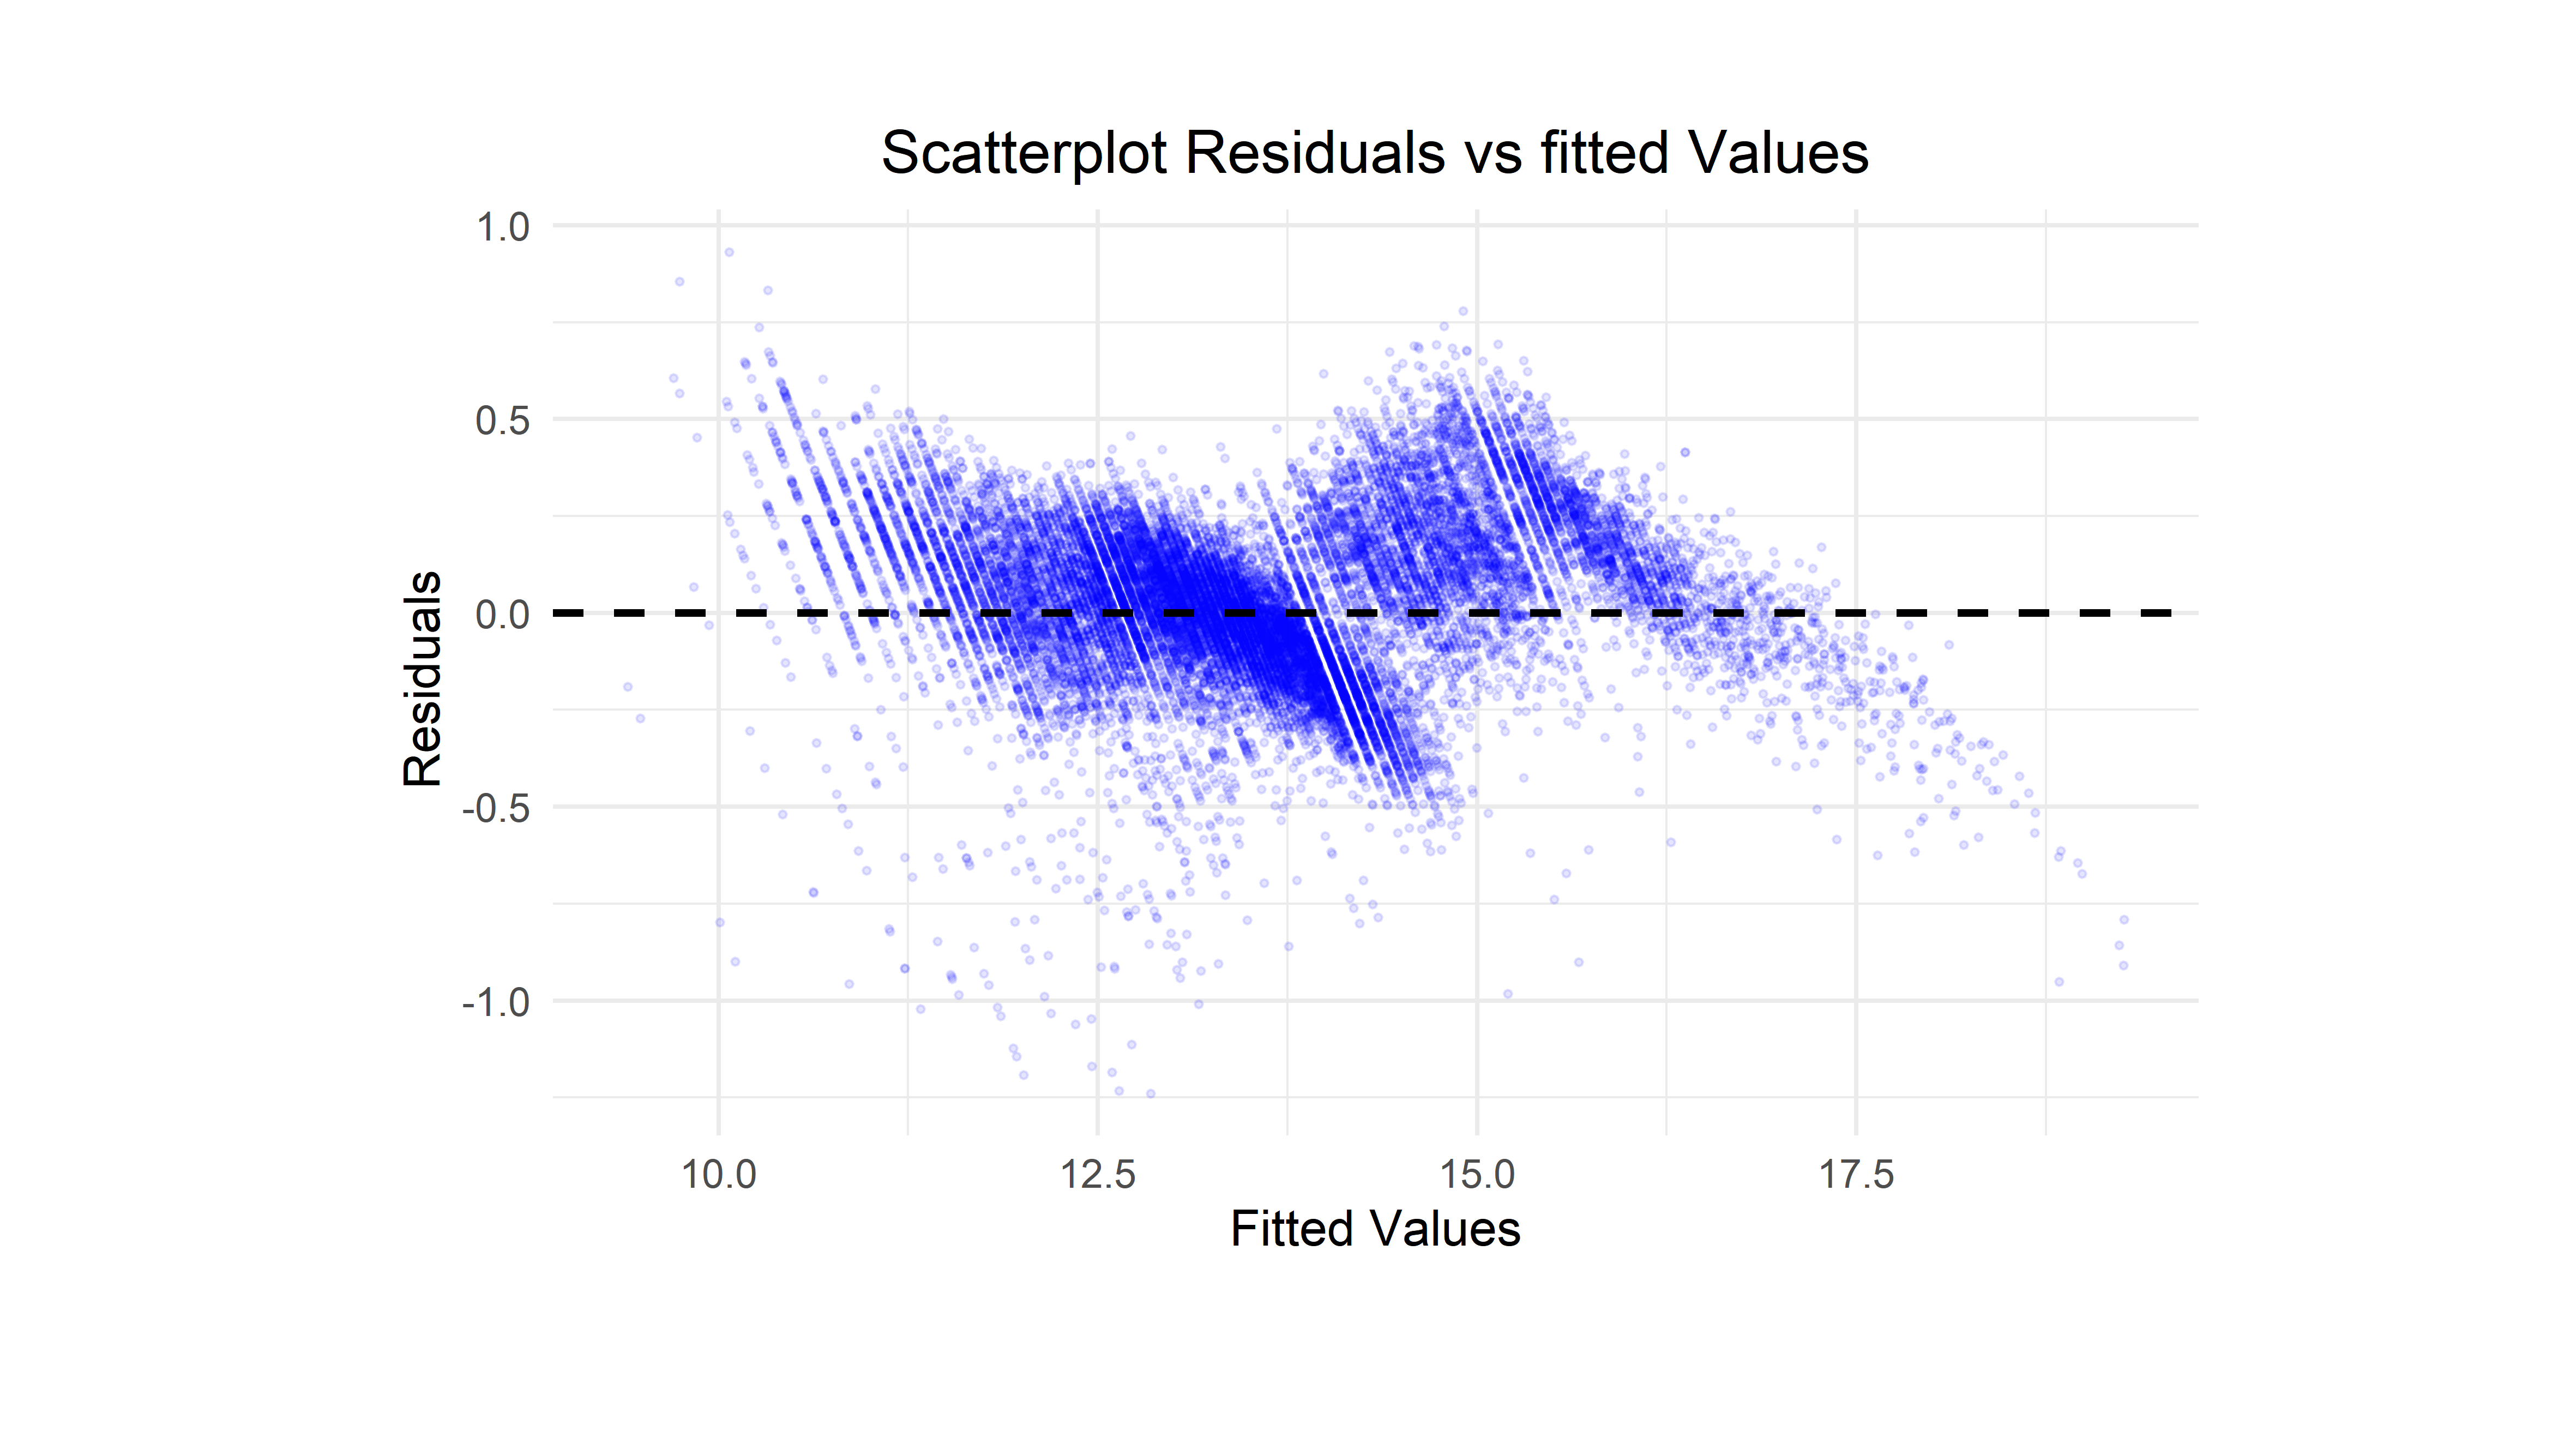
\includegraphics[width=1\linewidth]{C:/Users/HP/Documents/GitHub/bayes/04_output/pl_bay_res} \hfill{}

\caption{ \label{fig:res_bay} Plot of the Residuals vs Fitted Values for the Bayesian LASSO}\label{fig:fig2}
\end{figure}

In Figure \ref{fig:res_bay} the residuals versus the fitted values were
plotted and it appears that several assumptions are violated, on a first
glance. On one hand it seems to be that there is a relationship between
fitted values and residuals. On the other hand, there also seem to be
clusters with different variances. The variance in the range between 10
and 13 seems to be larger than the variance between 15 and 18, which
could be a sign for heteroscedasticity.

Furthermore, the model seems to have a systematic estimation error for
high values, all estimated values above 16 have a naegative residuum,
i.e.~the model overestimates the value of the players. Generally, it can
be said that a pattern can be recognized and the residuals do not appear
distributed independently of each other.

\begin{figure}

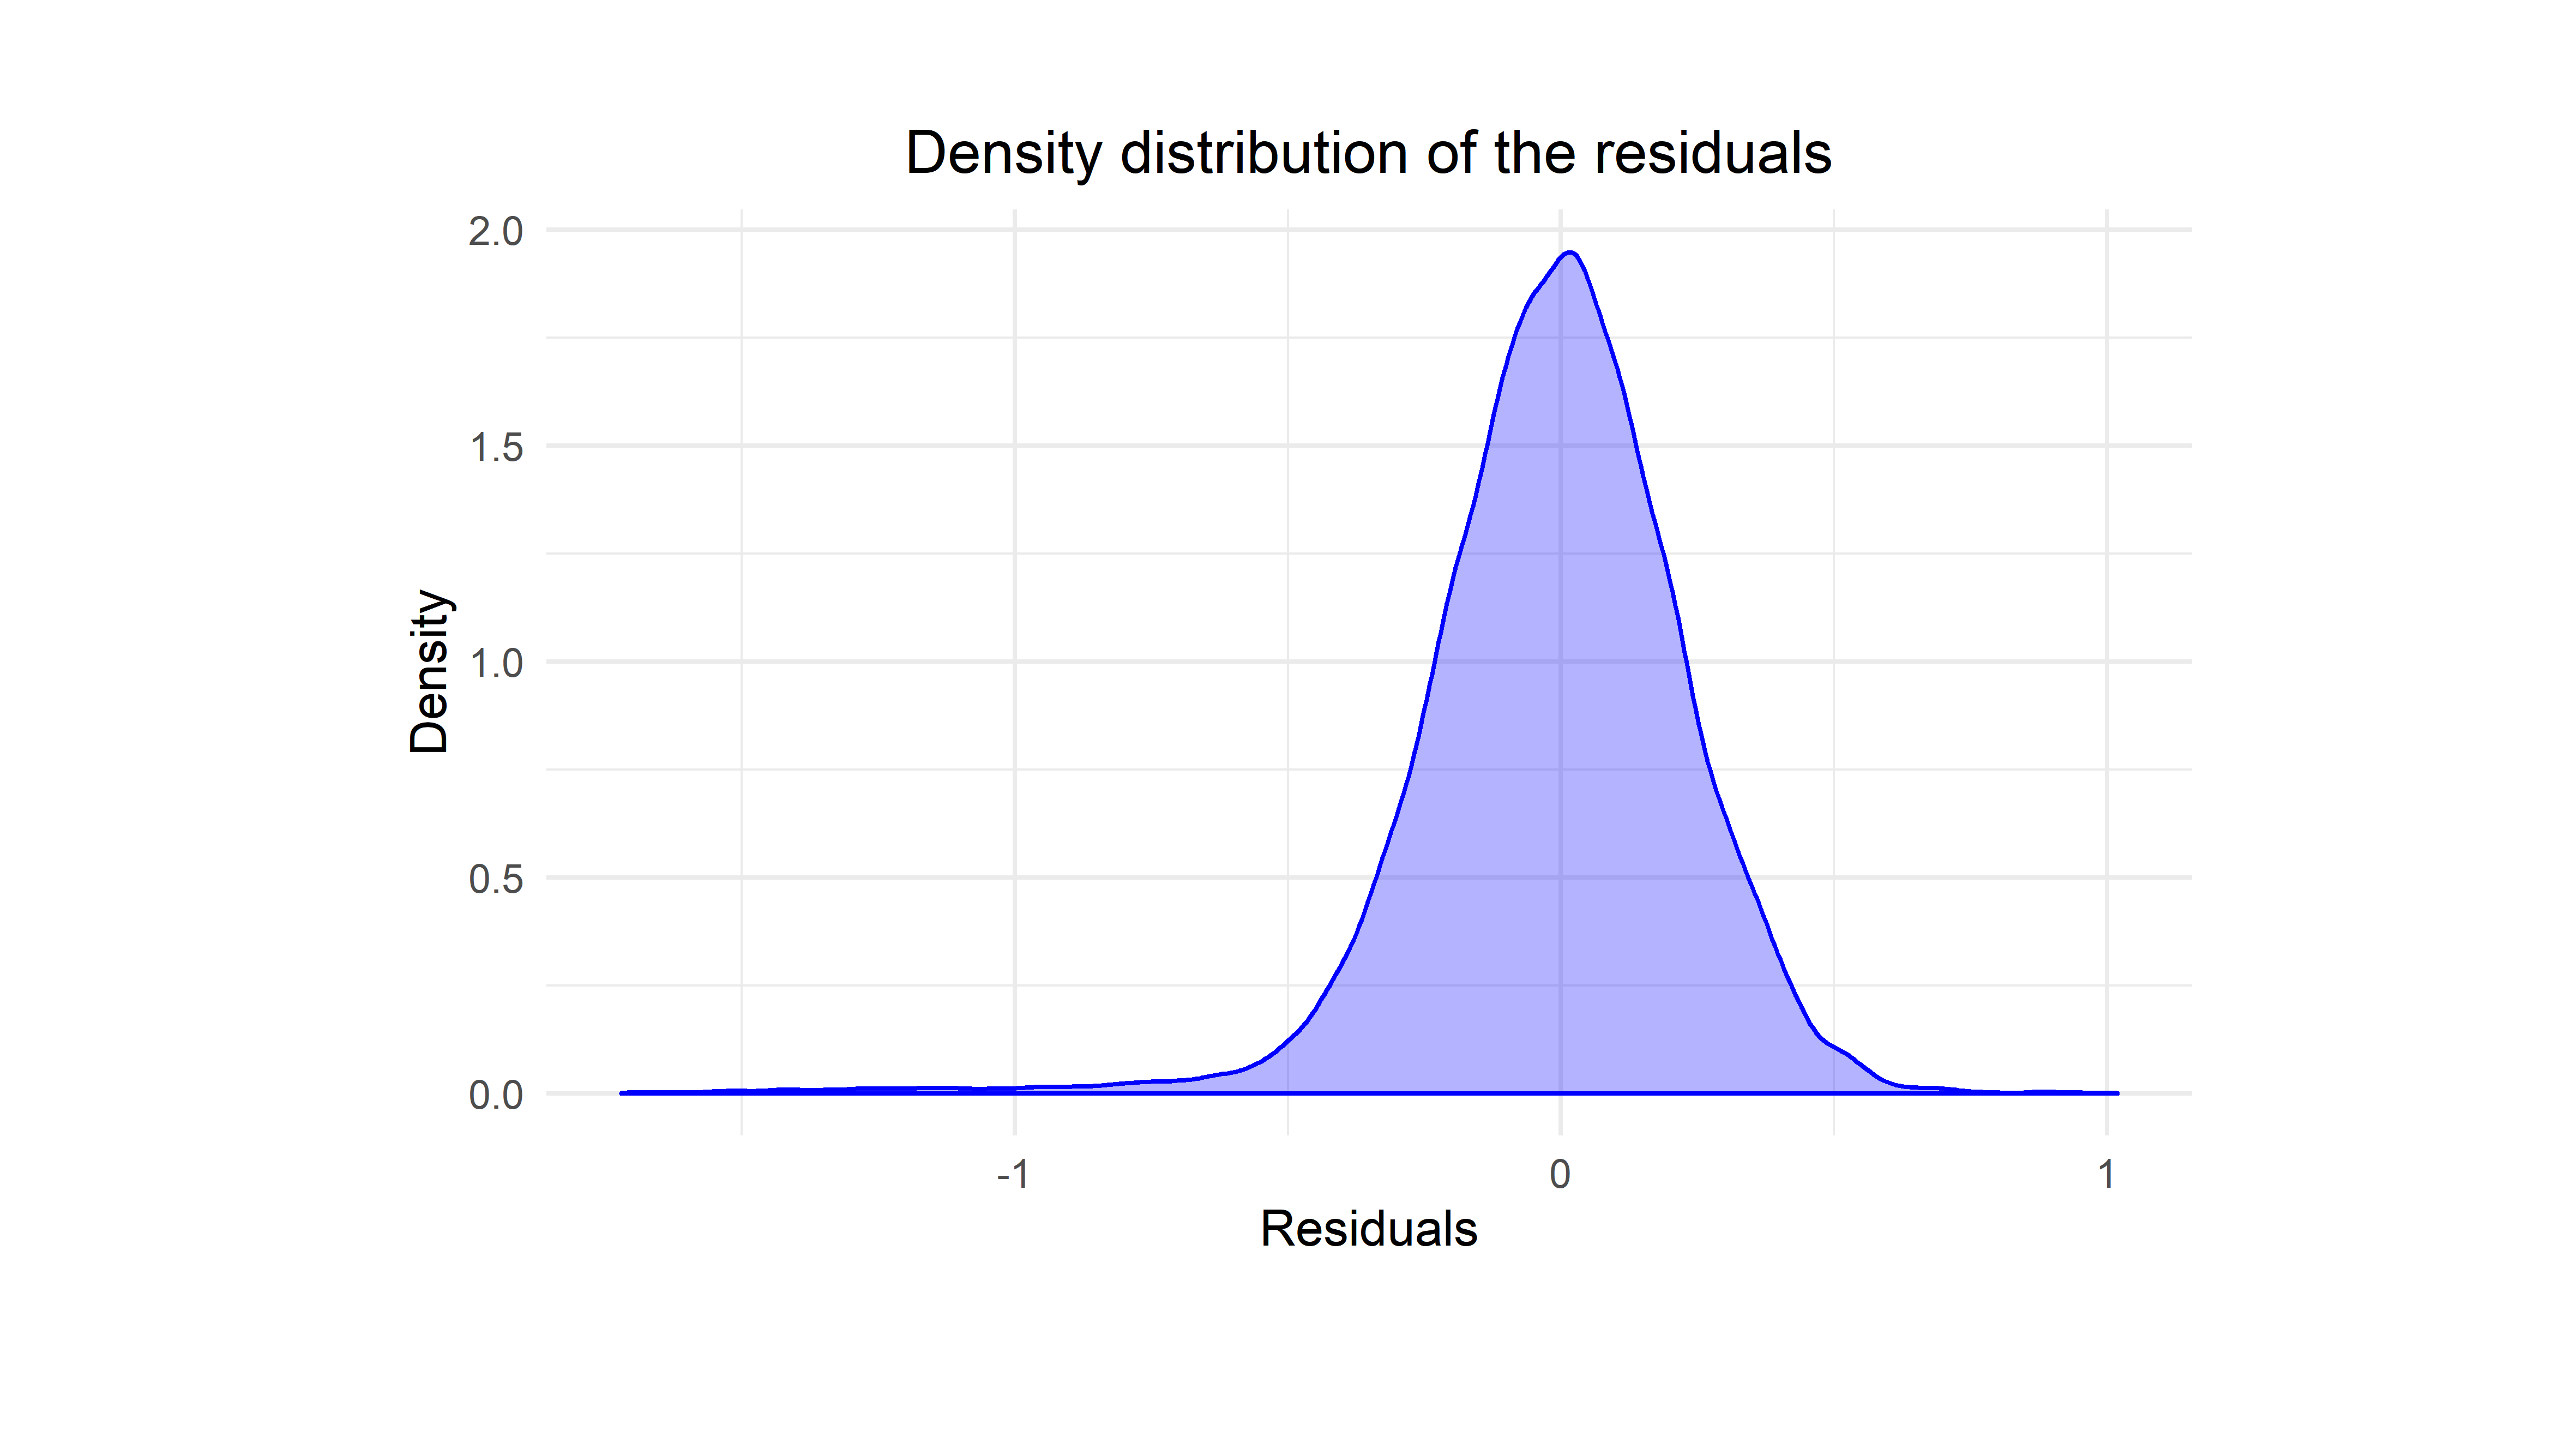
\includegraphics[width=1\linewidth]{C:/Users/HP/Documents/GitHub/bayes/04_output/pl_bay_res_dens} \hfill{}

\caption{ \label{fig:den_res_bay} Distribution of the Residuals of the Bayesian LASSO}\label{fig:fig_dens_2}
\end{figure}

The distribution of the residuals also does not seem to be normally
distributed with a mean value of 0. In Figure \ref{fig:den_res_bay} it
seems that the left tail is much longer and wider than the right tail.

The empirical mean of the residuals is -0.0138247, which is significant
different to zero at a one percent level with a t-static of -7.63 and a
p-value of 2.50e-14. For the residuals of the \ac{OLS} and the
\ac{LASSO} model, the observations are the same, as shown in Figures
\ref{fig:res_lm} and \ref{fig:res_lm_dens} for the \ac{OLS} model and
Figure \ref{fig:res_lasso} and \ref{fig:res_lasso_dens} for the
\ac{LASSO} model in the Appendix.

Since the \acf{OLS} method is our base method for the comparison and we
are mainly interested in comparing the number of parameters included (or
excluded) in (from) the model. Therefore, the \ac{OLS} model was
estimated again with corrected standard errors for heteroscedasticity.

First of all, we performed a Breusch-Pagan test for heteroscedasticity
which was significant to a 5\% level with a BP score of 2640.89 and a
p-value of \(\approx\) 0.00e+00 and the non-constant variance score test
of Breusch-Pagan test was also significant to a 5\% level test with a
\(\chi^2\) score of 42.1247 and a p-value of
\ensuremath{8.5636553\times 10^{-11}}.

With the corrected standard errors, 2 coefficients are no longer
significant, which is 1 coefficient more as in the first \ac{OLS} model.

\hypertarget{of-the-models}{%
\subsection{\texorpdfstring{\acf{RMSE} of the
Models}{ of the Models}}\label{of-the-models}}

As already mentioned in the introduction, we have taken the \emph{FIFA}
data from \emph{2020} as test data. At least briefly, it should be noted
here that the leap from the 2019 edition to the 2020 edition has added a
further dimension. Between the two years there could be a trend, which
could catch other effects like inflation, that increases player values
without being explained by any of the variables in the model.

In a quick check using a linear \ac{OLS} model containing the data for
both years and a dummy for the different versions, we get a significant
estimator of 0.0322. This estimator is significant with corrected
standard errors at a significance level of 5 percent with a t-value of
13.967 and a p-value of 3.37e-44.

The significant dummy for the \emph{versions} does not automatically
mean that there is an annual trend. The main thing to keep in mind is
that we excluded a number of variables at the beginning and that these
can now be included in the dummy as a bias.

However, all three models have the same problem and therefore this
should not play a major role in the RMSE's assessment of the models. The
RMSE should therefore increase equally for all three models. The
\acf{RMSE} is calculated as follows:

\begin{align*} 
  RMSE = \sqrt{ \dfrac{ \displaystyle \sum_{i = 1}^{N} \left( \hat{y}_i  - y_i \right)^2} {N}    }
\end{align*}

The \ac{RMSE} is a relative comparison measure that calculates the
performance of different models using the same data set. If the
\ac{RMSE} is determined with other data, as in this case with the 2020
data, it is called an out-of-sample RMSE.

The RMSE for the frequentist linear model is 0.218308, which in itself
is difficult to interpret. For the (frequentist) LASSO, the RMSE is
0.217305, which is a reduction of -0.46 percent compared to the base
linear regression.

For the Bayesian \ac{LASSO}, which was estimated with \(12.500\)
\ac{MCMC} iterations, \(2.500\) of which were cut off at the beginning
and were not used for the calculation. We get a \ac{RMSE} of 0.216686,
which is a change to \ac{OLS} of -0.74 percent. Compared to the
frequentist \ac{LASSO} we get a reduction of the RMSE of -0.28 percent.

The improvement in the \ac{RMSE} of the Bayesian model compared to the
linear model is relatively small and is even smaller compared to the
\ac{LASSO}. However, the computational effort for the small improvement
is relatively high. The linear model (with corrected standard errors)
was calculated within a few seconds. Whereas the frequentist \ac{LASSO}
took only slightly longer, despite the cross-validation for the
punishment parameter \(\lambda\), the Bayesian \ac{LASSO} took almost 18
hours due to the 12.500 \ac{MCMC} iterations.

\hypertarget{changing-other-hyperparameter}{%
\subsection{Changing other
Hyperparameter}\label{changing-other-hyperparameter}}

As \textcite{park_bayesian_2008} have described in their paper, instead
of selecting \(\lambda\) directly, one can also use a diffuse prior and
only specify the parameters of the gamma distribution. We took the
proposed parameters from \textcite{park_bayesian_2008} with \(r = 1\)
and \(\delta = 1.78\).

\FloatBarrier
\begin{table}[!h]

\caption{\label{tab:sensity }\label{tab:sum_bay_hy_1} Summary of the  Bayessian LASSO with hyperpriors}
\centering
\begin{tabular}[t]{lrrr}
\toprule
  & median & 2.5\% & 97.5\%\\
\midrule
\rowcolor{gray!6}  log\_wage & 0.067611 & 0.062648 & 0.072639\\
age & -0.100563 & -0.102264 & -0.098894\\
\rowcolor{gray!6}  height\_cm & 0.001243 & 0.000000 & 0.001957\\
weight\_kg & 0.000000 & 0.000000 & 0.000479\\
\rowcolor{gray!6}  overall & 0.209864 & 0.208337 & 0.211426\\
potential & -0.005909 & -0.007363 & -0.004507\\
\rowcolor{gray!6}  shooting & 0.004825 & 0.004257 & 0.005428\\
contract\_valid\_until & 0.004740 & 0.000000 & 0.007845\\
\rowcolor{gray!6}  pace & 0.000623 & 0.000000 & 0.001137\\
passing & 0.001612 & 0.000000 & 0.002577\\
\rowcolor{gray!6}  dribbling & -0.001330 & -0.002459 & 0.000000\\
defending & -0.001601 & -0.001924 & -0.001163\\
\rowcolor{gray!6}  variance & 0.057674 & 0.056483 & 0.058891\\
lambda.square & 0.000089 & 0.000023 & 0.000261\\
\bottomrule
\end{tabular}
\end{table}
\FloatBarrier

As Table \ref{tab:sum_bay_hy_1} shows, the results have not really
changed. There are still 6 parameters outside the 95 percent credibility
interval and, also the size of the effects have hardly changed, which is
mainly due to the many iterations of the \c{MCMC} algorithm. Also, the
\(\lambda\)-parameter differs only slightly , from 1.24e-04 to 8.94e-05.
The respective 95 percent credibility intervals overlap, which means
that they are not differ significantly.

\newpage

\hypertarget{conclusion}{%
\section{Conclusion}\label{conclusion}}

As we have shown in sections 5 and 6, the results of the Bayesian
\ac{LASSO} are very similar to the results of the frequentist
\ac{LASSO}. However, the Bayesian \ac{LASSO} performs a bit better,
measured by the \ac{RMSE}, which does not seem to be substantially
different. Our results are similar to those of
\textcite{park_bayesian_2008}, who also found no great difference
between Bayesian LASSO and the normal one. However,
\textcite{hans_bayesian_2009} found a reduction of the average
prediction error from 16 to 36 percent with different dataets.

The small difference in the methods can - of course - also be due to the
underlying data, since we estimate and calculate the RMSE with only one
data set. As we have seen from the analyses of the residuals and the
distribution of the response variable, the data are not optimal either.
A possibility for further analysis would be a Box-Cox transformation of
the data to see if the Bayesian LASSO has greater advantages. Another
possibility would be to generate data with a Monte Carlo simulation and
then let the different methods do the estimation again. In this way,
certain problems - such as heteroskedasticity - can be controlled.

\newpage

\hypertarget{appendix}{%
\section{Appendix}\label{appendix}}

\(\quad\)

\begin{figure}

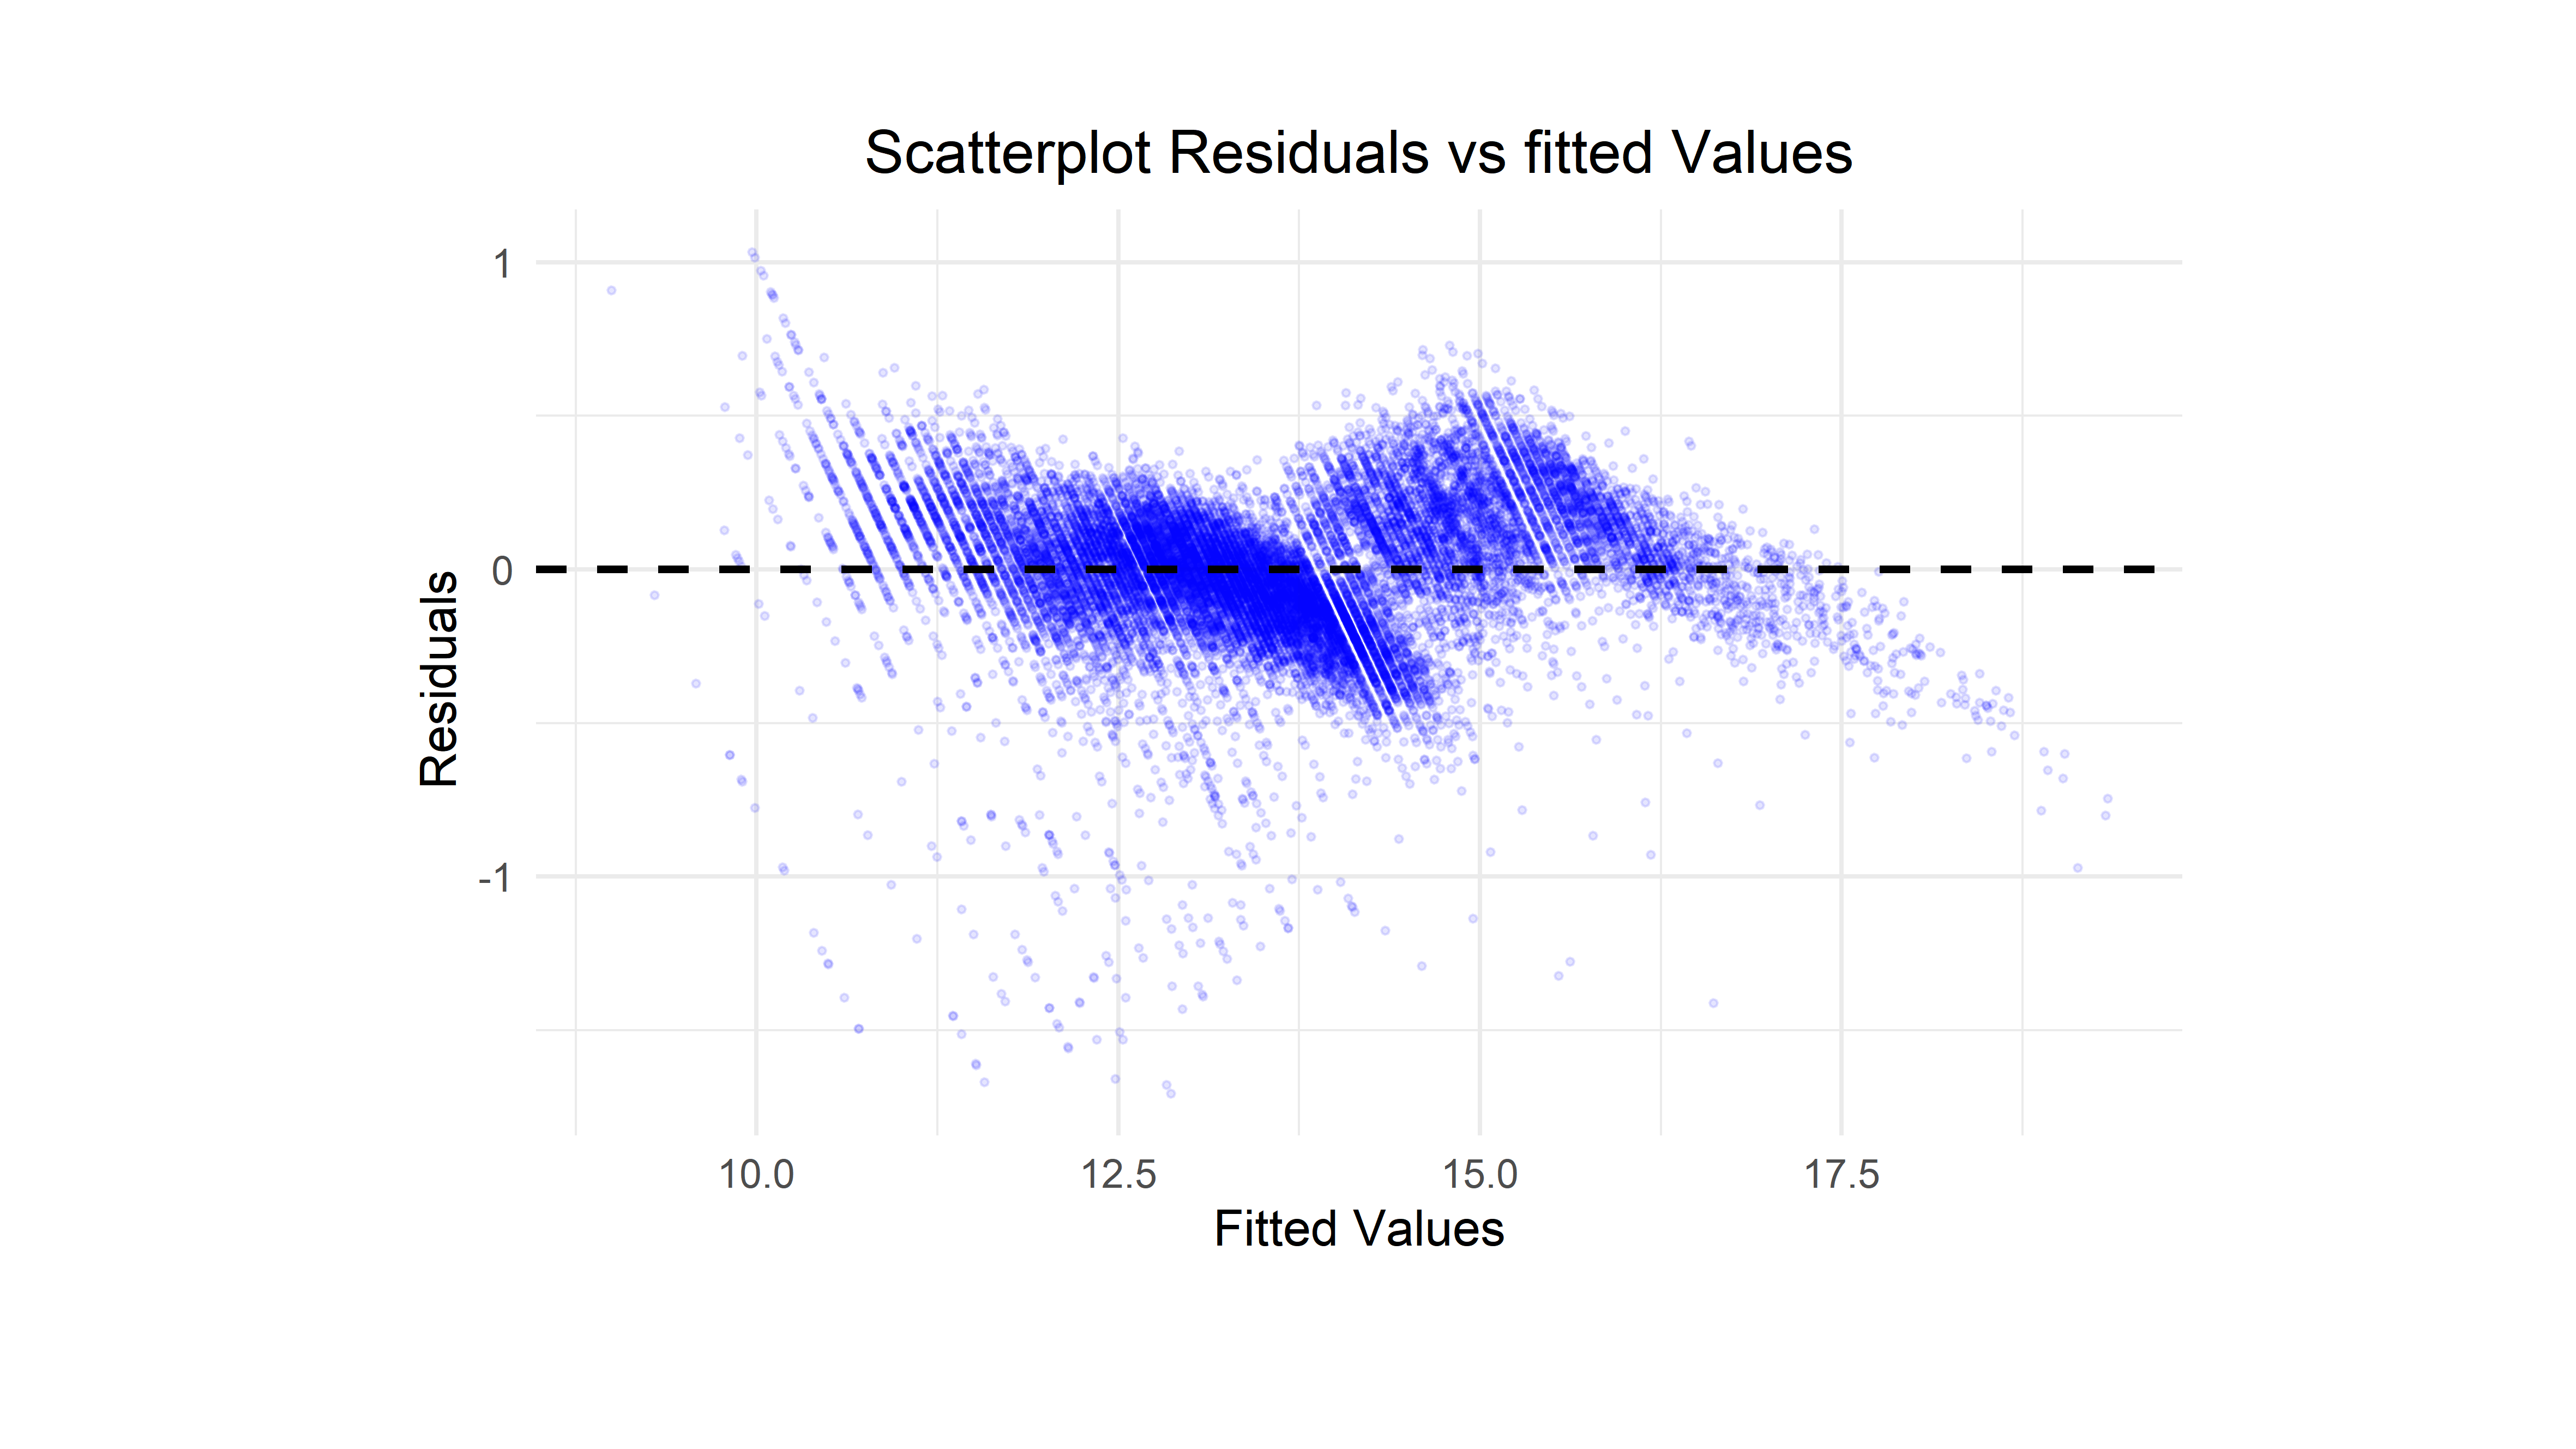
\includegraphics[width=1\linewidth]{C:/Users/HP/Documents/GitHub/bayes/04_output/pl_lin_res} \hfill{}

\caption{ \label{fig:res_lm} Plot of the Residuals vs Fitted Values for the Linear Model}\label{fig:fig3}
\end{figure}

\begin{figure}

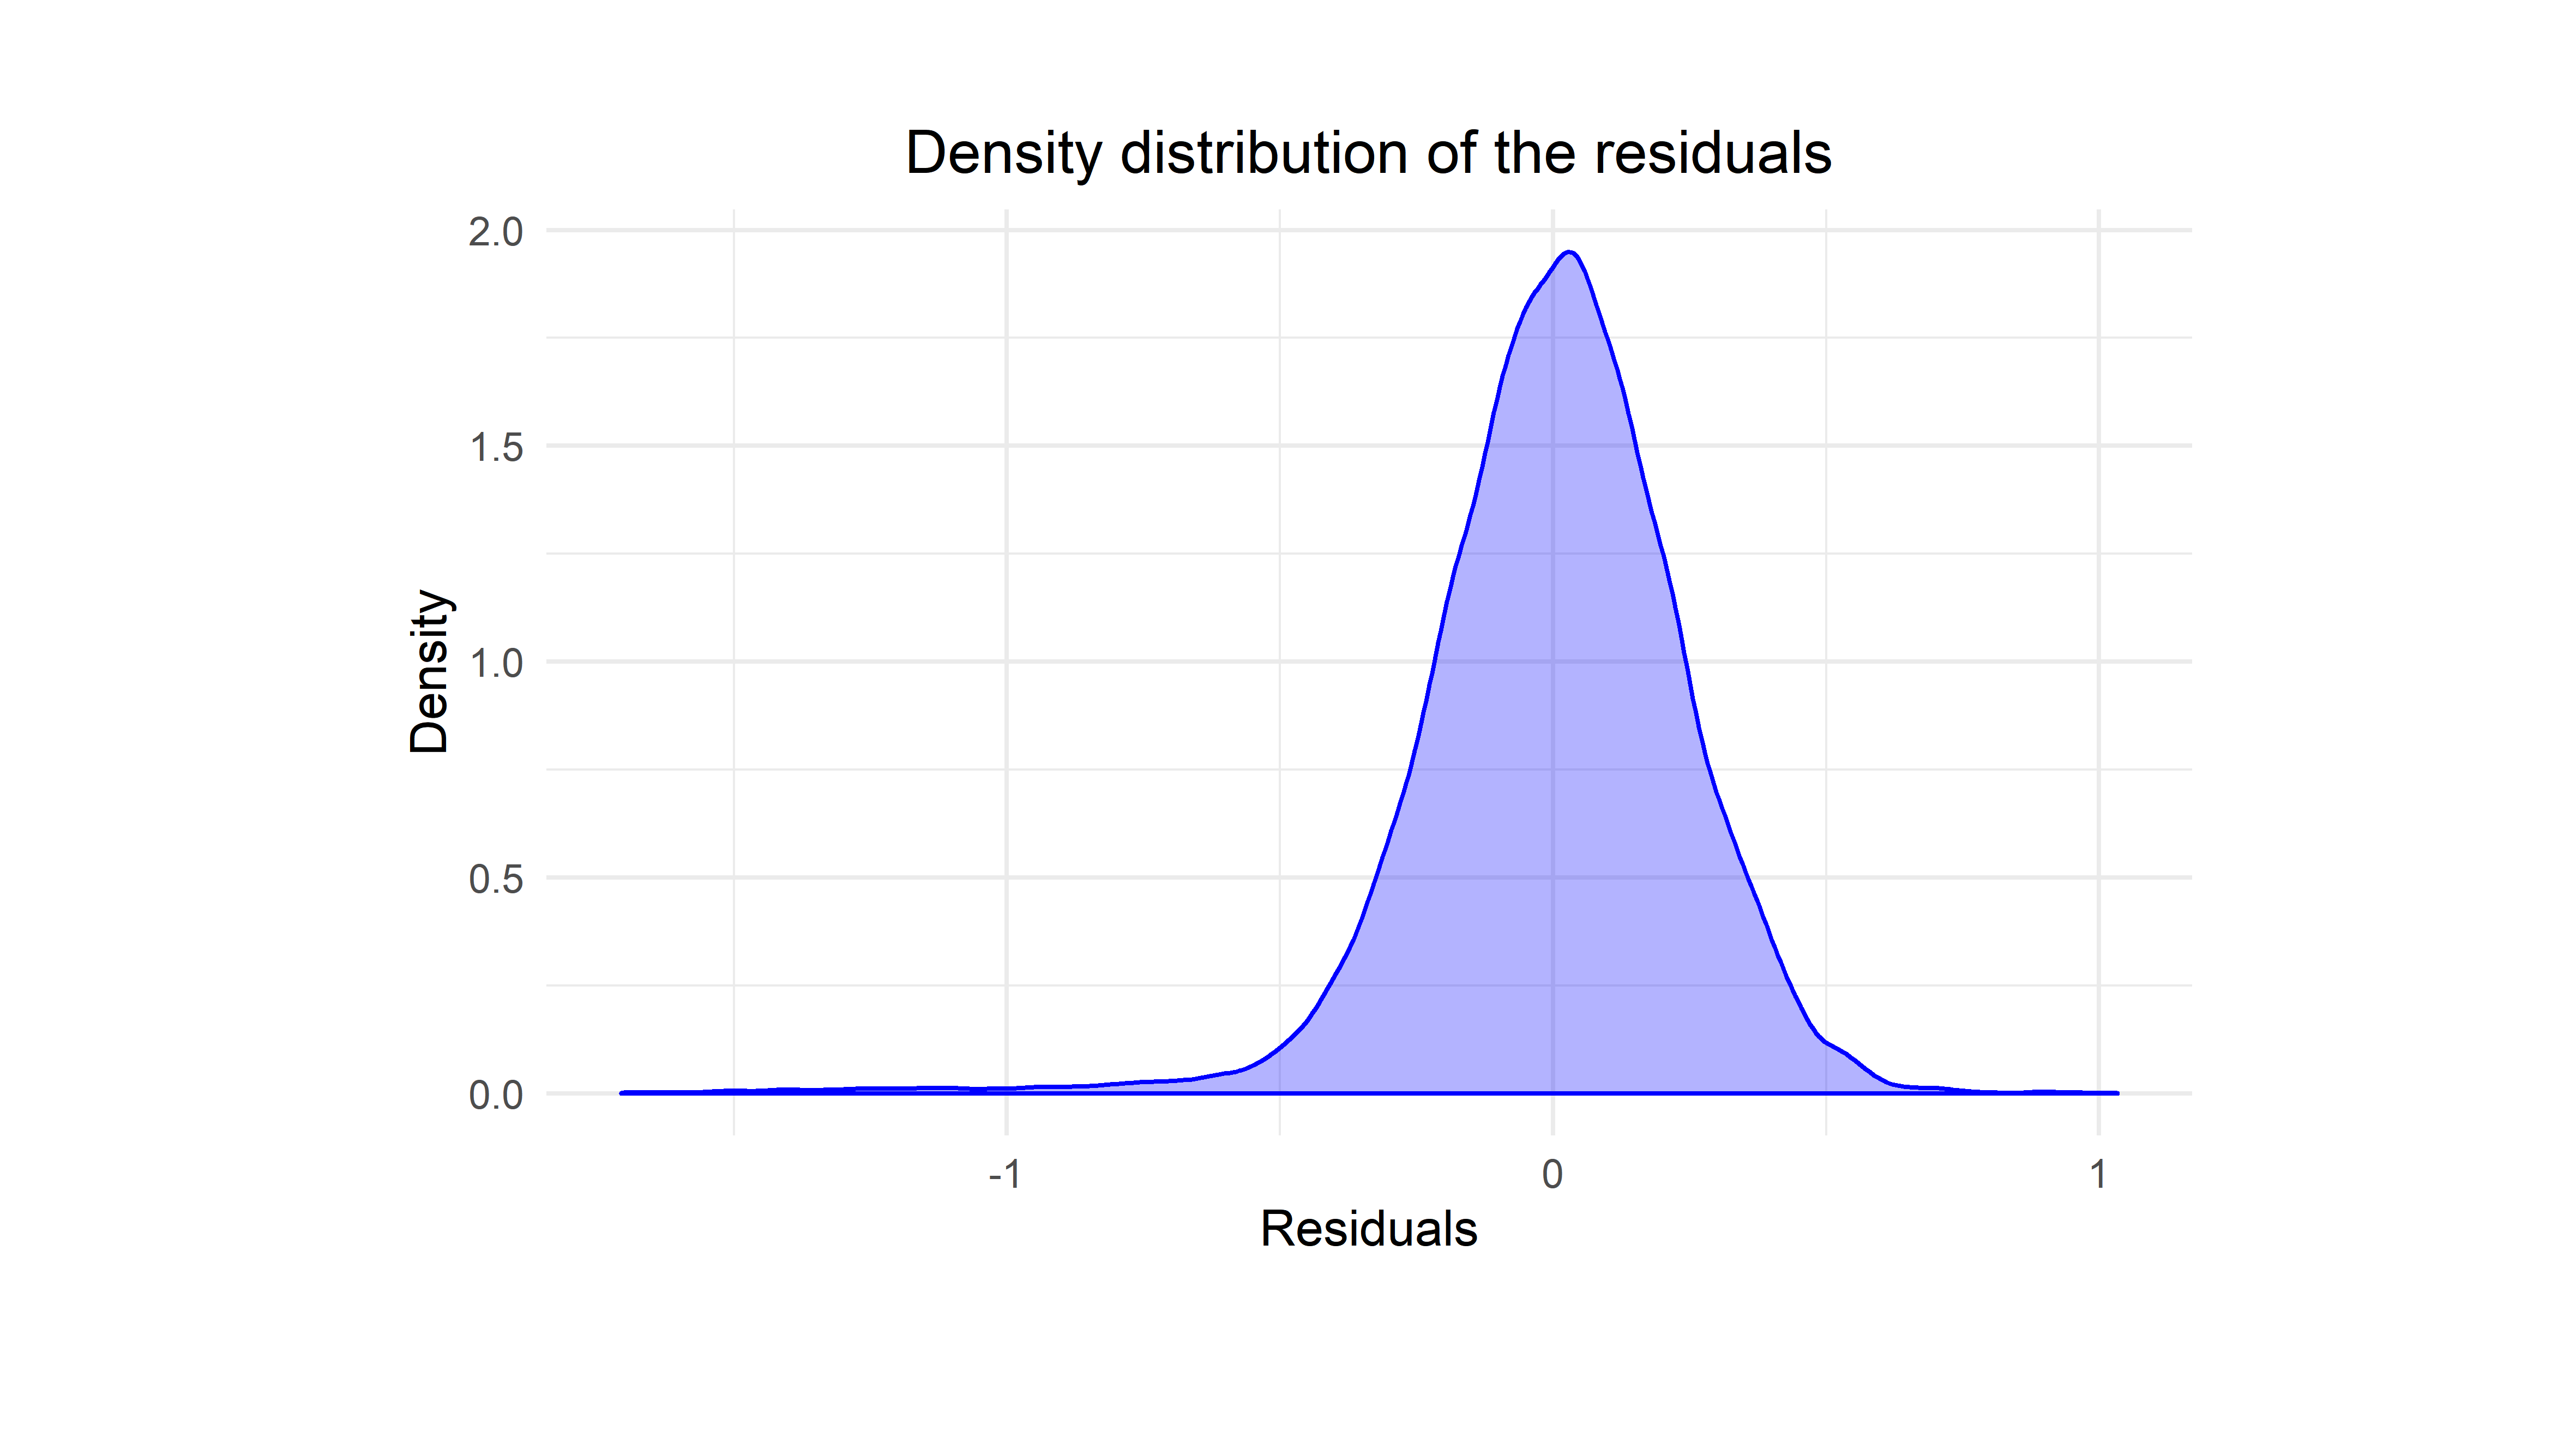
\includegraphics[width=1\linewidth]{C:/Users/HP/Documents/GitHub/bayes/04_output/pl_lm_res_dens} \hfill{}

\caption{ \label{fig:res_lm_dens} Density Plot of the Residuals of the Linear Model}\label{fig:fig3_dens}
\end{figure}

\newpage

\begin{figure}

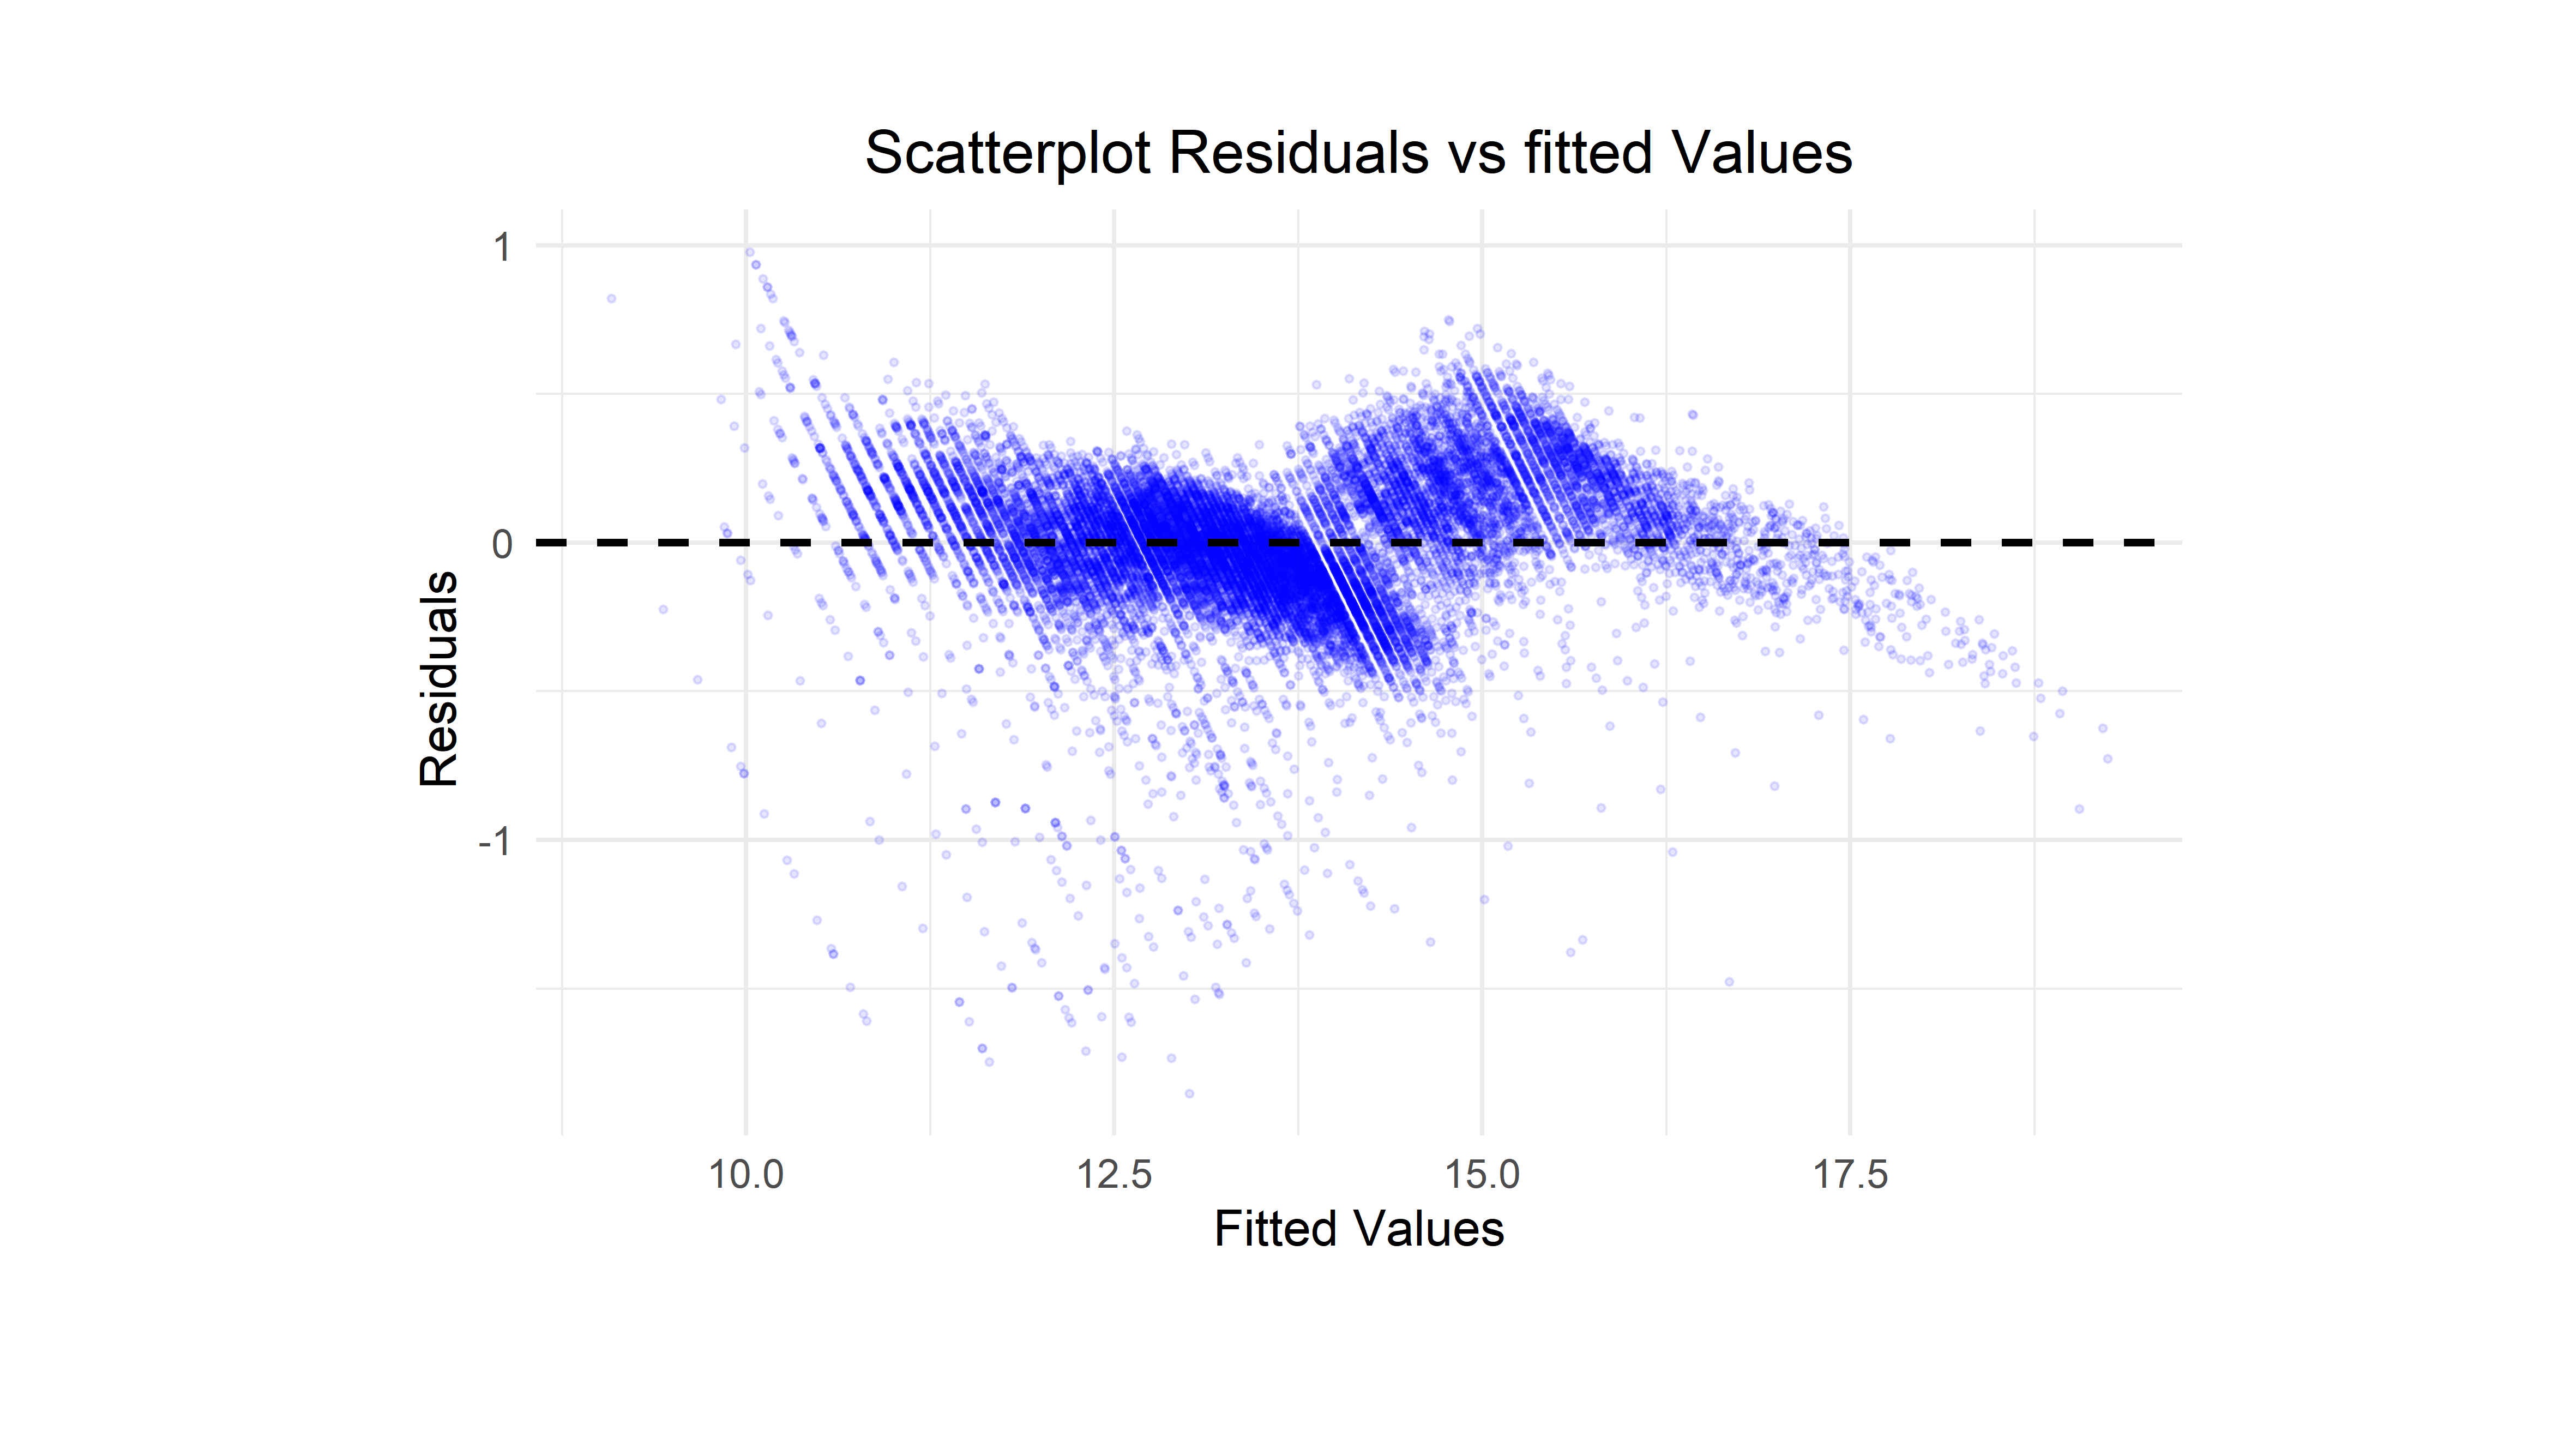
\includegraphics[width=1\linewidth]{C:/Users/HP/Documents/GitHub/bayes/04_output/pl_las_res} \hfill{}

\caption{ \label{fig:res_lasso} Plot of the Residuals vs Fitted Values for the LASSO Model}\label{fig:fig4}
\end{figure}

\begin{figure}

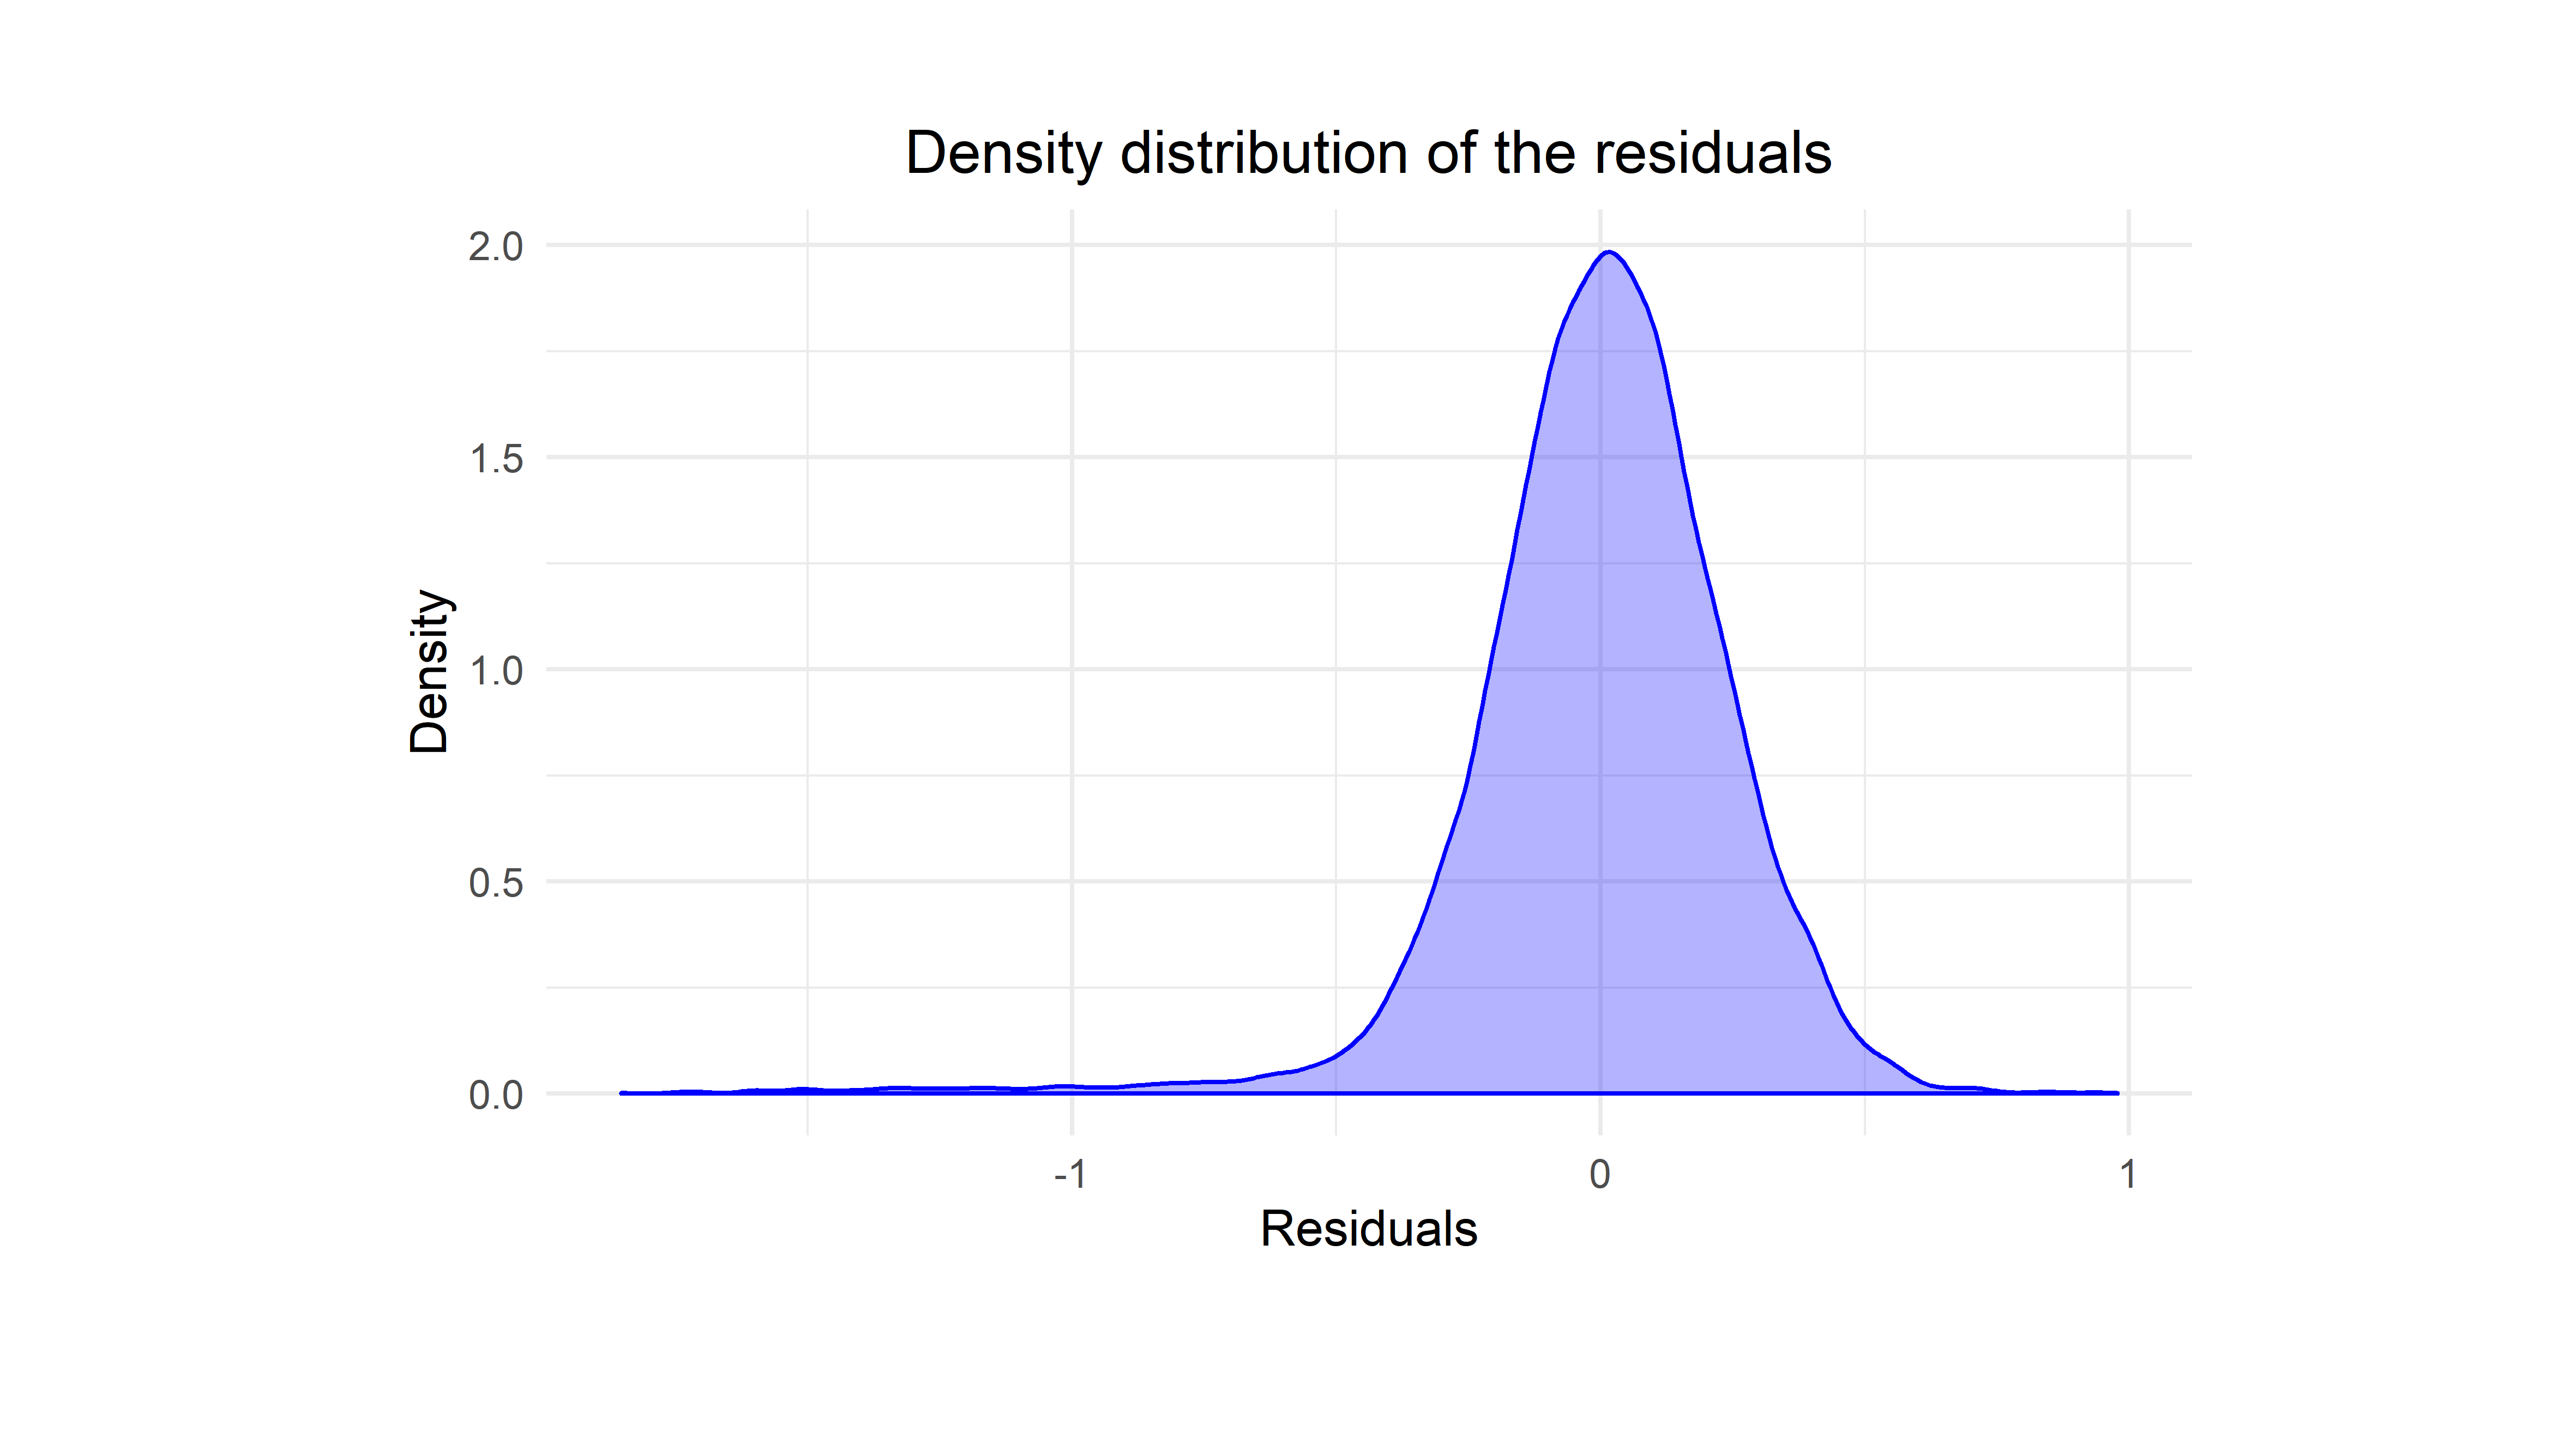
\includegraphics[width=1\linewidth]{C:/Users/HP/Documents/GitHub/bayes/04_output/pl_las_res_dens} \hfill{}

\caption{ \label{fig:res_lasso_dens} Density Plot of the Residuals of the LASSO Model}\label{fig:fig4_dens}
\end{figure}

\newpage
\newpage
\renewcommand*{\mkbibnamefamily}[1]{\textbf{#1}}
\renewcommand*{\mkbibnamegiven}[1]{\textbf{#1}}
\renewcommand*{\mkbibnameprefix}[1]{\textbf{#1}}
\renewcommand*{\mkbibnamesuffix}[1]{\textbf{#1}}


\printbibliography[title=References]
\pagenumbering{arabic}


\newpage
\textbf{Eidesstattliche Versicherung}

\bigskip

Ich versichere an Eides statt durch meine Unterschrift, dass ich die vorstehende Arbeit selbständig und ohne fremde Hilfe angefertigt und alle Stellen, die ich wörtlich oder annähernd wörtlich aus Veröffentlichungen entnommen habe, als solche kenntlich gemacht habe, mich auch keiner anderen als der angegebenen Literatur oder sonstiger Hilfsmittel bedient habe. Die Arbeit hat in dieser oder ähnlicher Form noch keiner anderen Prüfungsbehörde vorgelegen.

\vspace{1cm}
\rule{0pt}{2\baselineskip} %
\par\noindent\makebox[2.25in]{\indent Essen, den \hrulefill} \hfill\makebox[2.25in]{\hrulefill}%
\par\noindent\makebox[2.25in][l]{} \hfill\makebox[2.25in][c]{Jens Klenke}%


\end{document}
